\documentclass[useAMS,usenatbib]{mn2e}
\bibliographystyle{mn2e}

\usepackage{amsmath}
\usepackage{commath}
\usepackage{hyperref}
\usepackage{graphicx}
\usepackage{natbib}
\usepackage{times}
\usepackage{float}
%\usepackage{caption}
\usepackage{subcaption}
\usepackage{multirow}
\usepackage{color,soul}
\usepackage{import}
\usepackage[T1]{fontenc}
\usepackage{ae,aecompl}
\usepackage{amssymb}	% Extra maths symbols
\usepackage{multicol}        % Multi-column entries in tables
\usepackage{bm}		% Bold maths symbols, including upright Greek
\usepackage{pdflscape}	% Landscape pages
%\usepackage{booktabs,fixltx2e}
\usepackage[flushleft]{threeparttable}


\newcommand \Spitzer {{\it Spitzer }}
\newcommand{\boldit}[1]{\textbf{\mathversion{bold}#1}}

\newcommand \aaj {A\&A}
\newcommand \aarv {A\&ARv}%: Astronomy and Astrophysics Review (the)
\newcommand \aas{A\&AS}%: Astronomy and Astrophysics Supplement Series
\newcommand \afz {Afz}%: Astrofizika
\newcommand \aj {AJ}%: Astronomical Journal (the)
\newcommand \apss {Ap\&SS}%: Astrophysics and Space Science
\newcommand \apj {ApJ}
\newcommand \apjs {ApJS}%: Astrophysical Journal Supplement Series (the)
\newcommand \araa {ARA\&A} %: Annual Review of Astronomy and Astrophysics
\newcommand \asp {ASP Conf. Ser.}%: Astronomy Society of the Pacific Conference Series
\newcommand \azh {Azh}%: Astronomicheskij Zhurnal
\newcommand \baas {BAAS}%: Bulletin of the American Astronomical Society
\newcommand \mem {Mem. RAS}%: Memoirs of the Royal Astronomical Society
\newcommand \mnassa {MNASSA}%: Monthly Notes of the Astronomical Society of Southern Africa
\newcommand \mnras {MNRAS} %: Monthly Notices of the Royal Astronomical Society
%\newcommand {Nature}%(do not abbreviate)
\newcommand \pasj {PASJ}%: Publications of the Astronomical Society of Japan
\newcommand \pasp {PASP}%: Publications of the Astronomical Society of the Pacific
\newcommand \qjras {QJRAS}%: Quarterly Journal of the Royal Astronomical Society
\newcommand \mex {Rev. Mex. Astron. Astrofis.}%: Revista Mexicana de Astronomia y Astrofisica
%\newcommand {Science }%}%(do not abbreviate)
\newcommand \sva {SvA}%: Soviet Astronomy
\newcommand \aap {APP} %:American Academy of Pediatrics
\newcommand \apjl {ApJL} %:The Astrophysical Journal Letters

%\defcitealias{Hossein12}{T12}

\begin{document}
% TITLE
\defcitealias{Hossein12}{T12}

\title[SOM: classifying high $Z$ galaxies]{Clustering galaxies at 0.5 < $z$ < 1: an unsupervised approach} %PB160426: suggest "Clustering galaxy spectra at $0.5<z<1$: an unsupervised approach" -- I think if you say "clustering galaxies" people will think of spatial clustering
\author{rahmani.sahar }
\date{\today}
\author[S.~Rahmani, H.~Teimoorinia and P.~Barmby]{S.~Rahmani$^{1}$\thanks{E-mail:
srahma49@uwo.ca}, H.~Teimoorinia$^{2}$, P.~Barmby$^{1}$\\
$^{1}$Department of Physics $\&$ Astronomy, Western University, London, ON N6A 3K7, Canada\\
$^{2}$Department of Physics $\&$ Astronomy, University of Victoria, Finnerty Road, Victoria, British Columbia, V8P 1A1, Canada}
\maketitle

%----------------------------------------------------------------------------------------
%----------------------------------------------------------------------------------------
%----------------------------------------------------------------------------------------
%abstract
%----------------------------------------------------------------------------------------
%----------------------------------------------------------------------------------------
%----------------------------------------------------------------------------------------

\begin{abstract}%% (Must be 250 Words)
% In this paper, we introduce a new method of clustering of high red-shift galaxies, based on their spectral energy distributions (SED)s. We use unsupervised self organizing map(SOM) to train an artificial neural network to categorize SEDs of galaxies. We utilize as spectral template as a training set, and trained networks to be able to clustered galaxies based on the template. We cluster a sample of 142 galaxies with 0.5< z <1 using the trained network. We train networks with various sizes and properties to investigate the nature of the 142 sample galaxies. For each network, we cluster the sample of 142 galaxies and visualise their properties. In order to test new classifications,we compare physical properties of the galaxies in each cluster. We compare our results with  clustering  results  from  other  artificial  neural  networks,  and  with  the  original template classification. We conclude that SOM is a very useful method to be used in classifying galaxies based on their SEDs. It can be used to find morphology of the high red-shift galaxies, and find a new class of SEDs.
In this paper, we introduce a new method of clustering high red-shift galaxies, based on their spectral energy distributions (SED)s.
%Artificial neural networks provide us a reliable method to cluster SEDs of galaxies.
We use an unsupervised self organizing map(SOM) as a training method to train networks with a sample of galaxies with SEDs between FUV to NIR wavelengths, which their morphological types are known.
Since information that can be extracted from each network depends on the size and dimension of the trained networks, in this project we train networks with different grids in 1D or 2D.%%???
We visualise each trained network using a new version of SOM plots.
To test trained networks, we cluster a sample of 142 galaxies with 0.5 < $z$ < 1 using each of the trained networks.
We plot average SED of SEDs of galaxies in each neuron in 1D networks, to investigate the nature of galaxies in new clusters.
For each network, we visualise the properties of galaxies in each neurons. %%%% combine 94 and 93 
We compare mean physical properties of the galaxies in each neuron such as age, specific star formation rate, stellar mass, and FUV extinction, with each other and found a tight correlations between them. 
Comparing our results with clustering results from supervised artificial neural networks, show us using SOM we can classify galaxies in between types of original spectral types. %%rephrase
As a result we have a power tool to classify spectra of galaxies based on their SEDs which also can  identify galaxies with a new shape of SEDs.

%%%% SR20160512: I do not like it! But I do not know how to fix it. I already wrote at least 4 version of it. I need help with this one:((

%%% what is the problem we are trying to solve in general! why do we want o classify thing in general, and what is wrong in exciting classification scheme

\end{abstract}
\begin{keywords} 
 galaxies: high red shifts, galaxies: spectral energy distribution, methods: observational, methods: statistical, data mining, methods:data analysis
\end{keywords}
%----------------------------------------------------------------------------------------
%----------------------------------------------------------------------------------------
%----------------------------------------------------------------------------------------
%Intro
%----------------------------------------------------------------------------------------
%----------------------------------------------------------------------------------------
%----------------------------------------------------------------------------------------
\section{Introduction}
\label{sec: intro}
%General information about SEDs
All information we can obtain from a galaxy is encapsulated in the light it emits; every observable phenomenon in a galaxy leaves a footprint on the spectral energy distribution (SED) of that galaxy.
We can determine some physical properties of galaxies by properly modeling various features observed in their SEDs.
The general shape of the SEDs can be used as an identifier of the morphological type of the galaxies.
Considering the main features of the SEDs galaxies can be categorized in two main groups: elliptical, or spiral.
Each group has its own characteristic features and can be divided into many sub-branches.

%%Creating templates and NIR_UV templates
Several attempts have been made to composite a thorough template for categorizing the spectral type of galaxies using data from nearby galaxies~\citep[e.g.][]{Kinney93}~\citep[][hereafter K96]{Kinney96}~\citep[][]{Bershady00,Mannucci01}. 
Based on their usage, these templates are restricted to certain wavelengths.
In near-infrared (NIR) to ultraviolet (UV) domain of wavelengths (the region where output of stars peaks), SED contains information about the main physical properties of galaxies, e.g., age, star formation rate (SFR), stellar mass, wide range of the stellar population, some information on interstellar medium (ISM)'s absorption and emission lines, and extinction from ISM of the galaxies.


% categorizing galaxies based on their SED

Attaining high-resolution data and detailed SEDs has been made possible due to advances in imaging techniques, and photometry and spectroscopy devices.
This has helped to see the more detailed SEDs, which made classification of galaxies more complex.
Since no two galaxies, even with the same morphology, have exactly the same properties, classifying the SED of the galaxies using the templates are a challenge.
Many fitting methods are developed and used to find the best matches of template for each SED.
$\chi^2$ minimizing method is the most commonly used method to do so. 
Artificial neural networks (ANNs), K-mean clustering, and principal component analysis are the other methods to cluster and classifying the morphological type of the galaxies based on their SED \citep[e.g.][]{Allen13,Ordov14,Shi15}.

%ANNs
ANNs are very powerful tools to use in data processing and pattern recognition problems.
Their information processing method was inspired by the way neurons in human brains work.
An ANN contains many interconnected units (nodes or neurons) which process data and work together to solve problems.
It uses a set of training methods to learn about a non-linear and complex relations between input and output data and how to apply it to new sets of data.
Studies show that ANNs provide better fitting than minimizing chi-squared and would be an alternative choice for fitting data~\citep[e.g.][]{Marquez91,Moayed09}.
In cases that both methods show the same correlation, ANNs still are a better method of fitting due to their faster results on large databases \citep[][]{Gulati97}.

%Training methods for networks
Neural networks can be trained using two methods; supervised and unsupervised.
In supervised method, a neural network would be trained using input data based on desired outcome.
This method is very useful for classification of data with specific target values (e.g. any pattern recognition with known templates).
On the other hand, in unsupervised method there is no prediction of output data.
This method classifies data based on their underlying structures and hidden variables.
The unsupervised method is a very helpful method to knowledge discovery of your data, or when the underlying structure of data is not well established (e.g. producing a template of SED of galaxies).

%SOM
Kohonen Self organizing map (or self organizing map, SOM) is an unsupervised neural network for mapping and visualizing a complex and non-linear high dimension data introduced by~\citep{Kohonen82}.
The SOM is a technique that shows a simple geometry relationship of a non-linear high dimension data on a map \citep{Kohonen98}.
%SOM in Astronomy
The utilization of the SOM in astronomy dates back to 1990s. 
\citet[][]{Odewahn92}, \citet[][]{Hernandez94}, and \citet[][]{Murtagh95} were among the first studies in astronomy that used SOM for their studies.
From classifying quasars' spectra to star/galaxy classifications, from gamma-ray bursts clustering to classification of light curves, this method have been used in various aspects in astronomy \citep[e.g.][]{Maehoenen95, Miller96,Andreon00,Balastegui01,Rajaniemi02,Brett04,Scaringi09}.
%20160509PB: suggest starting a new paragraph here, with an introductory sentence about galaxy spectra.
%SR20160512: I start new paragraph after the next sentence not here.
\citet{Geach12} used COSMOS data to demonstrate two of main applications of SOMs; object classification and clustering, and photometric redshift estimation. 
The later one was subject of many studies \citep[e.g.][]{Kind14a}.

%SOM in Astronomy continued.
Spectrum of a galaxy is a combination of spectra of million stars and clouds inside the galaxy.
Therefore, large spectra data sets contain information of billions of stars and other objects inside galaxies, and needs to be studied carefully. %%%EEEHHHH
\citet{In12} introduced a new clustering tool, which is based on the SOM method for analysing large data of spectra.
They used $\sim 60000$ spectra from the Sloan Digital Sky Survey \citep[SDSS;][]{Abazajian09}
to test their tool, and created very large SOMs to analyse the type of spectra/objects.
They also generated SOMs from quasars' spectra in order to find unusual types of quasars' spectra. Later \citet{Meusinger16} used these SOMs and updated data from SDSS and other surveys and found a new class of quasars.
The other application of the SOM is to find outliers or errors in the data.
\citet{Fustes13} produced a package based on SOM to classify spectra from GAIA survey that were previously classified as "unknown" by SDSS pipeline. The package recognizes an astronomical object from artificial errors, and then classifies the object based on its spectra.

%What T12 did
~\citet[][hereafter T12]{Hossein12} classified SEDs of this sample of galaxies using supervised neural network method, based on the spectral template presented by K96.
With supervised method, they could only classify SED of the 105 out of 142 galaxies.
The SED of the 37 galaxies from their samples could not be matched with any of those in the K96 templates. 
In order to classify the remaining 37 galaxies, they combined spectrum of the K96 templates.
This procedure showed that, not a single type of galaxies in K96 template could describe the SED of any of those 37 galaxies.
Since the SOM have the freedom of classifying objects in between the known classes, it be applied on this data to find the best SED class for the 37 galaxies.
T12 also showed that there are tight correlations between physical properties of galaxies and these correlations might be different for each type of the galaxies.

%What we did
In order to compare supervised and unsupervised methods directly, we used exactly the same data as T12 used.  
First, we trained SOMs using data from K96 and compared our classification with K96 galaxies classification.
Then, we used the trained network to classify the SEDs of 142 galaxies with 0.5 < $z$ < 1 from T12 paper.
Same as T12, We also plotted the properties of the T12 galaxies based on the new clusters and compared them with previuse works.
In Section $\S$~\ref{sec: data}, we present the data that we used to train and test our networks. We describe the SOM methos in Section $\S$~\ref{sec: method}. The results of the SED classifications and comparing them with previous studies are shown in Section $\S$~\ref{sec: result}. In Section $\S$~\ref{sec: summary}, we present the summary of our results and the future works in this subject.

%----------------------------------------------------------------------------------------
%----------------------------------------------------------------------------------------
%----------------------------------------------------------------------------------------
%DATA
%----------------------------------------------------------------------------------------
%----------------------------------------------------------------------------------------
%----------------------------------------------------------------------------------------

\section{DATA}
\label{sec: data}
We used SED templates from K96, to train neural networks.
To test the trained networks, we used SED and physical properties of 142 galaxies at 0.5 < $z$ < 1 from T12.
Following of T12 work, we chose these two sets of data to not only show the application of SOMs in SED clustering, but also to easily compare both supervised and unsupervised methods.

 \subsection{Kinney spectral model}
     \begin{figure}
        \centering
        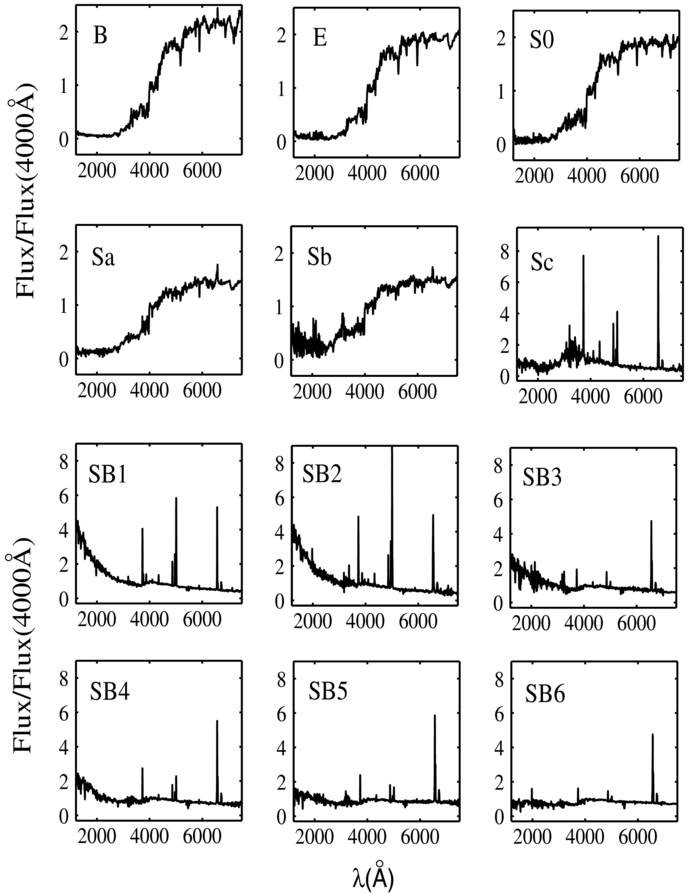
\includegraphics[width=0.5\textwidth]{images/k96.jpg}
        \caption{K96 spectra template for 12 types of galaxies from T12 paper (Fig. 1 in T12).Type of each template is shown in each frame. Plots B, E, S0, Sa, Sb and SC show spectra that belongs to early type galaxies. Starburst galaxies spectra are indicated with SB 1 to 6. Higher numbers represent more intrinsic colour extinction.}
        \label{fig: k96}
    \end{figure}
      
    K96 used UV-optical spectra of 70 star forming and quiescent nearby galaxies to produce a template that contains 12 types of SEDs.
    These templates are widely used in many studies to determine morphological type of galaxies, or find properties of specific types of galaxies in many studies \citep[e.g.][]{Shakouri16,Paiano16,Laporte16,Holden16}.
    K96 mentioned that one of the usage of these templates can be classifying the SED of the high redshift galaxies. 
    The 12 types of spectra are divided based on their morphological types for early type galaxies or their extinction for starburst galaxies (Fig.~\ref{fig: k96}). 

    The quiescent group of galaxies includes Bulge (B), Elliptical (E), S0, Sa, Sb, and Sc galaxies.
    Bulge group represents galaxies similar to M31 and M81, which their UV and optical spectroscopy dominated by the stellar population in their bulges.
    
    The starburst galaxies are divided into six groups (SB1 - SB6) based on their intrinsic extinctions ($E(B-V)$). 
    As it is clear in the Fig.~\ref{fig: k96}, SB1 galaxies have lower internal extinctions ($E(B-V) \simeq 0.05$), while SB6 galaxies have the highest amount of extinction ($E(B-V) \simeq 0.65$) among starburst galaxies. 
    
    K96 spectra spans from $\sim1200-10000$\AA with resolution of $\sim 10$\AA~.
    However, we only used data between $\sim1200-8000$\AA~to train our networks. 
    This wavelength range was chosen due to availability of flux information in those wavelengths for all 12 types of galaxies.
    In early type galaxies' spectra (B to Sb), the spectrum is redder and strong absorption lines, and 4000\AA~break is distinguishable. 
    While SEDs of starburst galaxies are more flat on the optical and NIR part than early type one and show strong emission lines.
    For more details on each spectral type, we encourage readers to see K96 and references therein. 
    

 \subsection{SED and Properties of the sample galaxies} 
    T12 selected 142 galaxies from the spectroscopic campaign of the ESO GOODS-South field.
    For each galaxy, robust spectroscopic redshift and photometry data from the Good-MUSIC catalogue had been known.
    The 142 galaxies had been selected in T12 due to availability of data from HST/ACS; VLA/ISAAC; and \Spitzer/MIPS and IRAC for whole galaxies. 
    Data from these instruments were necessary in order to have a complete picture of stellar population and SFR.
    The photometry data contain information of the galaxies in 10 - 13 filters with the wavelength range of $\sim 0.4-24 \mu$m in the observed frame.
    T12 matched the resolution of the photometry data with K96 data and used these photometry data as inputs for Code Investigating GALaxy Enmission ({\em CIGALE} code;~\citep[][hereafter N09]{Noll09}) to generate the best fitted SED for each galaxy.% as well as some of the physical properties of the galaxies.
    
    {\em CIGALE} is a valuable tool to investigate the properties of the galaxy using UV to IR wavebands.
    It uses stellar populations, synthetic attenuation and dust emission models, spectral line templates, and active galactic nuclei's optical spectral templates to model SED of the galaxies.
    This code was successfully tested on data from 39 galaxies selected from the Spitzer Infrared Nearby Galaxy Survey (SINGS;~\citep{Kennicutt03}) by N09.
    T12 produced the best SED match, with wavelength interval of 910 to $\sim 8E9$\AA~, for each galaxy.
    Assuming decreasing SFR and visual attenuation ($\tau$) model, Salpeter initial mass function~\citep{Salpeter55} and old stellar population with age of $\sim 10$~Gyr, they derived physical properties of galaxies such as age, and stellar mass.
    Some of these properties are shown in Tab~\ref{tab: props}.
    In the Sec.~\ref{sec: 1D}, we studied these properties for each categorization.
    More details on creating SEDs and extracting information about galaxies properties using {\em CIGALE} can be found in N09 and T12.
    
       
    \begin{table}
\caption[]{Description of the properties of T12 galaxies; the output result of {\em CIGALE}}     
\label{tab: props}
\centering
\begin{tabular}{l l l}
\hline\hline
\noalign{\smallskip}
Par. & Unit & Description\\
\noalign{\smallskip}
\hline
\noalign{\smallskip}
$t_{\,\mathrm{oSP}}$ & Gyr & age of old SP model \\
$t_{\,\mathrm{ySP}}$ & Gyr & age of young SP model \\
$f_\mathrm{burst}$ & --- & mass fraction of \\
& & young single population (SP) model \\
\noalign{\smallskip}
$t_{\,\mathrm{D4000}}$ & Gyr & D4000-related age \\
\noalign{\smallskip}
$M_\mathrm{star}$ & M$_\odot$ & total stellar mass  \\
SFR & M$_\odot$/yr & instantaneous SFR  \\
$A_\mathrm{FUV}$ & mag & attenuation at 1500\,\AA{} \\
\noalign{\smallskip}
\hline
\end{tabular}
\end{table}

    For testing the created networks, we used SEDs that were produced by T12. 
    These SEDs are publicly available in the form of flux per rest frame wavelength in a wide range of wavelengths.
    Since we have used the T12 SEDs to test trained network, we only used the part of the SEDs that have a same wavelength range as K96 templates.  
 
 %%%%SR160611: The following is the Hossein's answers to the questions that you asked in the data section; Since, we did not used the spectra data here (we only used generated SEDs and information that was derived from SEDs) ,I assumed it is unnecessary to talk a lot about spectroscopy data. But, if you think it would help to understand the subject better, I will add those information to data section.


%  Is the data vector for each object a list of fluxes (flux densities) as a function of (rest) wavelength? I think we discus this question so I skip it.
%  Same wavelengths for every object? Yes
%  What is the spectral resolution? It depends on the type of spectra we use in T12 see
% below for more information.
%  Do the spectra include the whole galaxy or just the central part? For observed 142
% galaxies: whole spectra because they are in high redshift. For K96 they are co-added
% spectra from different parts.
%  Does the resolution match with K96? We match them to K96, see below.
%  What is the coverage of spectra? See below.
%  Do these galaxies have spectroscopic redshifts, or were redshifts derived from
%   photometry?" All 142 galaxies have robust spectroscopic redshift.
% For more clarification about spectra used in T12: We have three sets of spectra.
% 1 – observed spectroscopic spectra. They are used just for extra independent validation; see figure 17 from T12. This validation is nothing to do with network validations. The useful wavelength range (of
% FORS2 spectrometer) is 4800−10 000 Å, the nominal resolution is R = λ/Δλ = 580, which corresponds to
% a spectral resolution of ∼13Å. We use only range [3500-5100] because all the 142 observed spectra have information in this interval (some of them have no spectral information in 8000A, for example). In T12 you can also find this that can help: “The rest-frame spectra of the sample all include spectral information
% ∼3500–5100 Å. This interval brackets the important features such as the 4000Å break and also the strong emission
% lines such as [O ii]λ3727, λHβ 4861, and [O iii] λλ4959, 5007. The spectroscopic data for the sample galaxies contain different spectral types from starbursts (with a flatter continuum and stronger emission lines) to early-type galaxies (with a redder continuum, strong absorption lines, and large 4000Å break.”
% 2- k96 Model spectra which are for training. The spectra cover the interval ∼1200–10000Å and have a resolution of∼10 Å. We use only interval 1200-7500A. because all the 12 K96 spectra have information in
% this interval (some of the spectra have no information in 9000A, for example).
% 3– The Maraston’s models (SEDs): For each galaxy (from 142) we obtain a best Maraston spectrum (SED) by fitting photometric data to the models. Mraston’s models range very extended wavelength interval (from UV to far IR) with different resolution in different part of a given spectrum. For example resolution in IR is 100A and in optical ~3-5A. The best resolution is related to the optical part (3-5A and we convert all to 10A i.e., to resolution of K69). We cut the best 142 spectra in interval [1200-7500] like K96 for ANN validation or test. (If we had spectral information for all K96 spectra in the interval 1200-10000A, for example, then we would cut all 142 SEDs in 1200- 10000A). So if you find a new training set (other than K96 which we talked about that in our skype chat) and if they had information in 1000-15000A, for example, then we would cut the SEDs in this new interval for validation.
% As a summary: as you know (better than me!) we use K96 as training set and 142 SEDs as validation (or test) set. When we obtain the class of each 142 galaxies (in fact 105 galaxies! You are improving this number to 142 in your paper) then we use 105 observed spectra to make figure 17 from T12. The co-added observed spectra in a certain class match with the associated K96 spectra in the same class (i.e., an independent validation).

%----------------------------------------------------------------------------------------
%----------------------------------------------------------------------------------------
%----------------------------------------------------------------------------------------
%Method
%----------------------------------------------------------------------------------------
%----------------------------------------------------------------------------------------
%----------------------------------------------------------------------------------------

\section{METHOD}
\label{sec: method}
 \subsection{Self Organizing Maps}
 \label{sec: som}
 
 The SOM is a clustering method which reduces the dimension of data to lower dimensions, usually 1 or 2D, while preserving topological features of the original data.
 Results of SOM contain nodes (neurons) that arranged in 1D or 2D arrays \citep{Kohonen98}. 
 
 Each node may contain one or more samples from input data and distance between nodes represents similarity or dissimilarity of underlying samples. 
 In the way that similar data are closer together in the array and the further nodes go from each other, the more dissimilarity appears between their samples.
 A weight vector ``\boldit{W}" with same dimension of the input data associates with each node which will be changed during the process and has a key factor in a position of nodes in the map.
 
 \cite{Geach12} presented the application of the SOM and demonstrate the algorithm of the SOM in detail. In this section we are going to talk briefly about the algorithm of the SOM, how we create our maps and a test model which will help to interpret our results. 
 \subsubsection{Algorithm of SOM} 
 \label{sec: algorithm}
     Assuming we have a data set which contains vectors, \boldit{V} $\in \Re^n$, and we want to map them on S1 by S2 map. 
     We start by creating S1 $\times$ S2 empty neurons. 
     The initial arrangement of these neurons depends on a map's topology provided by users.
     In the case of the 1D maps, since each neuron has two immediate neighbours the topology of the map does not have any effect on the final result and we can choose any topology.
     However, in 2D maps, the shape of the neurons specifies the number of the immediate neighbours for each neuron and it is up to user that which shape is more suitable for their data.
     In this paper, we chose hexagonal topology which gives each neuron six neighbours, and causes more interactions between neurons.
     Then, a random weight vector, \boldit{W} $\in \Re^n$, will be assigned to each node.
     The process of creating SOM, happens over series of $N$ iterations. 
     During each iteration the weight vectors might change according to the Kohonen learning rule (equation~\ref{equ: weight adj}). 
      In each iteration SOM code:
     \begin{enumerate}
        \item Chooses a random vector from our data set ($V_i$).
        \item Calculates the Euclidean distance for each node, $j$, as  $D_j^2= \sum_{i=0}^{i=n} (V_i - W_i)^2$, and finds a neuron with minimum $D_j$, (``$D_{j_{min}}$"). This neuron is the winner node and is called the Best Matching Unit (BMU). 
        \item  Computes the radius of the neighbourhood of the BMU to find nodes within this radius. The weight vectors of these nodes will be affected in the next steps. This value is arbitrary and initially can be set to be as high as half of the SOM size and then it decades exponentially over each iteration:
        \begin{equation}
            r^t_{BMU} = r^0_{BMU}e^{(-t/\tau)}
        \end{equation}
        where $\tau$ is a decay constant and usually set to be the same as the number of iterations, $N$. $r^0_{BMU}$ and $r^t_{BMU}$ is the radius of the neighbourhood at 0th and $t$th iteration, respectively. 
        \item Changes the weight vectors of the BMU, and all the nodes within $r^t_{BMU}$ as:
        \begin{equation}
            \label{equ: weight adj}
            w(t+1)=w(t)+L(t) \times R(t) \times(v(t)-w(t))
        \end{equation}
        where $L(t) = L_0 e^{(-t/\tau)}$ is the learning factor which prevents divergence of the SOM and $R(t)=\exp(-\frac{D_j^2}{2r^t_{BMU}})$ is the influence rate. $R(t)$ determines how the weight of nodes in the neighbourhood of BMU will change.
        \item  Repeats these steps for $N$ times.
     \end{enumerate}
     
\subsection{Creating SOM}
\label{sec: create_som}
     In order to create SOM, we used {\tiny MATLAB} neural network 
     toolbox~\citep[NNT,][]{matlabtolbox}.
     %%Sr160611: Last time I got the following note from the MNRAS editor:
     %"Please note that computer software/programming lan- guages must be styled in SMALL CAPITAL LETTERS, according to journal style. Please check and correct this paper accordingly."
     SOM in {\tiny NNT} can be created by {\tiny NEWSOM} or {\tiny SELFORGMAP} library which both work in two phases. 
     Phase one is the ``ordering phase". 
     This phase starts with maximum neighbourhood distance, and initial high learning factor usually 0.9 which is provided by the user. 
     The ordering phase continues for the requested number of iterations.
     During the iterations, the learning factor reduces to tuning phase leaning factor and the neighbourhood distance reaches to tuning phase neighbourhood distance which both of the numbers set by the user.
     In the ordering phase, the changes in the learning factor and the neighbourhood distance adjust with the number of the iterations, in the way that at the last iteration, these two values reach to the initial values for the second phase.
     
     The second phase is the ``tuning phase".
     In this phase the neighbourhood distance is at its minimum, but learning factor decreases very slowly.
     This minimum neighbourhood distance and slowly decreasing the leaning factor helps to fine tune the topology results and causes the more stable SOM. 
     The number of iterations in this tuning phase most be much more than the number iterations in ordering phase, to allow the tuning to happen slowly. %cite kohenen book?!
     We chose the number of epochs the tuning phase to be 3 times more than the number of epochs in the ordering phase.
     
     To show our results, we used two of the {\tiny NNT}'s built-in plots.
     These plots, which are evolved version of old SOM plots, are designed to show distance between each clusters more clear.
     A Hits map, which shows the number of the times each neuron become the winner (hits), and a distance map, which shows the same neurons as the hits map and the distance between them.
     In the maps, the purple hexagonal shape areas represent the neurons.
     The distances in a distance map are shown by the grey cycle colours.
     The darker colour represents the larger distance between neurons; whilst the lighter colours means there is a small distance between neurons.
     In hit maps, neurons with zero hit left empty.
      
    Size of SOM maps is arbitrary and there is no rules or restrictions on choosing the size of the maps. 
    Although \cite{Vesanto05} suggested that the total number of  $5\sqrt{n}$ neurons provides the most sufficient size, users usually choose the size of grids based on their data set and their usages of the results.

   
\subsection{Mock sample}
 
         \begin{figure}
            \begin{subfigure}[b]{0.5\textwidth}
                \centering
                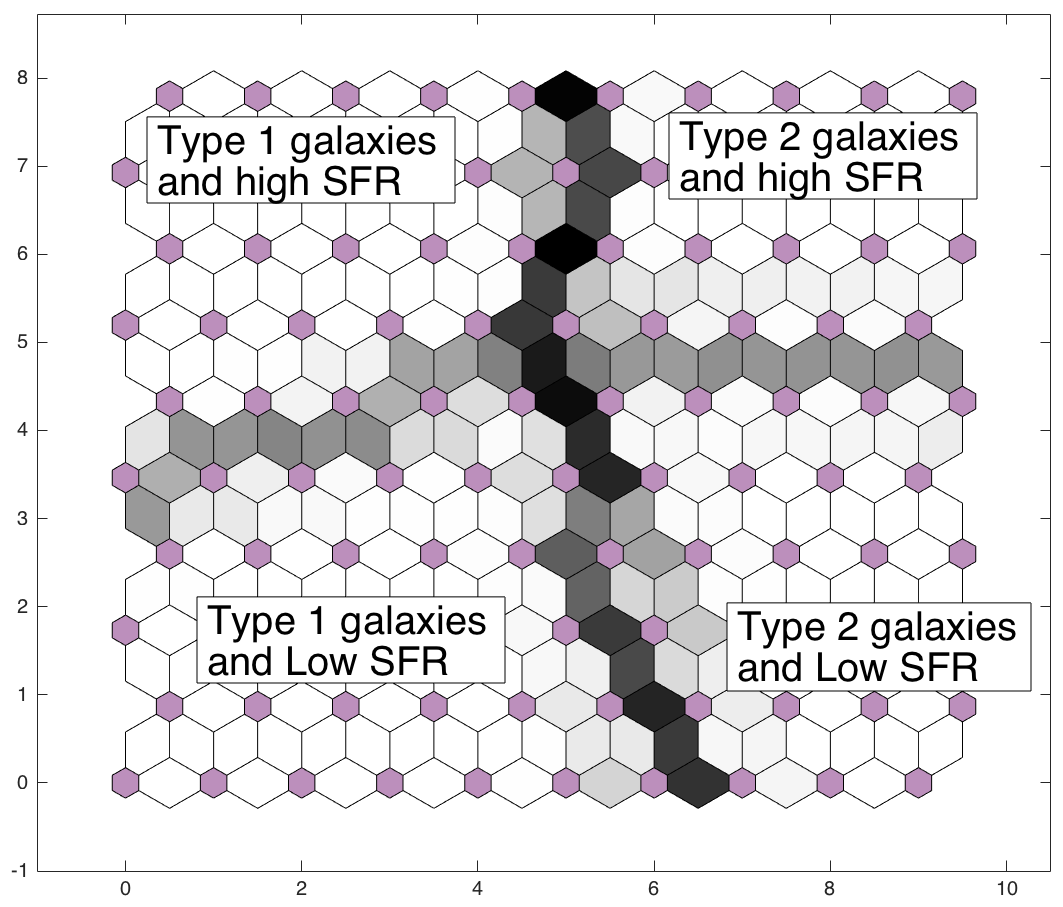
\includegraphics[width=\textwidth]{images0.01/sample/sample2_dist.png}
            \end{subfigure}
            \hfill
            \begin{subfigure}[b]{0.5\textwidth}
                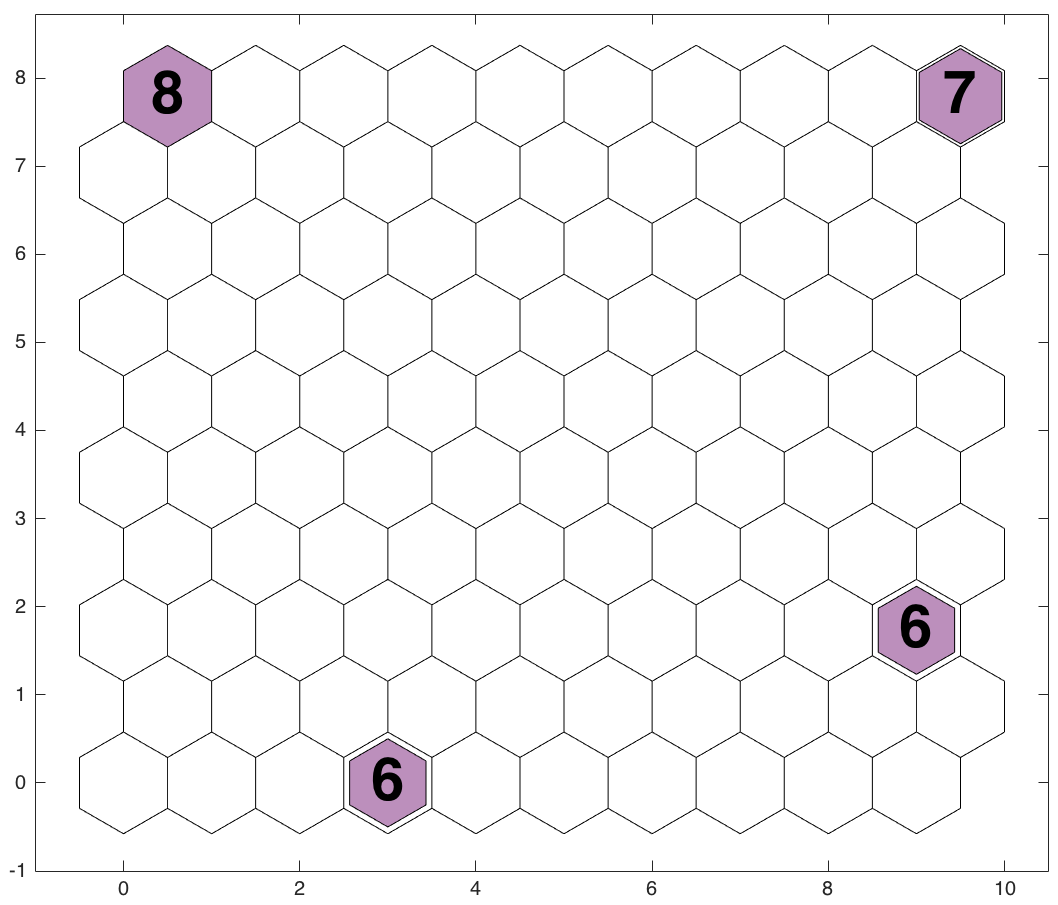
\includegraphics[width=\textwidth]{images0.01/sample/sample2_hits.png}
            \end{subfigure}
            \caption{SOM of the mock sample. In both plots, the axes show the position of the neurons. Hexagonal shapes represent the neurons. The upper plot is a distance map. The grey cycle colours show the differences between weight of each neuron with white is the minimum differences and black has the maximum one. The lower plot is a hit plot. It represents the number of samples in each neuron, while the empty with neurons means zero hit. In this sample the 27 galaxies clustered in 4 groups of 8, 7, 6 and 6 galaxies.}
            \label{fig: sample}
        \end{figure}
 
 We created  a mock sample of 27 galaxies to show how this method works, illustrate the results of SOMs, and how they can be analysed.
 The mock sample contains two information from each galaxy; The type of galaxies: type 1 or type 2, and either they are high or low star forming galaxies. 
 We generated a SOM with the size of $10 \times 10$ using the same initial values mentioned in the Section ~\ref{sec: create_som}.

 Fig. ~\ref{fig: sample} shows the SOM of the mock sample. 
 The upper plot is a distance map. 
 The axes show the position of the neurons in a $10 \times 10$ network.
 The lower plot in the Fig.~\ref{fig: sample} shows a hit map.
 On this map similar to the distance map the axes show the position of the neurons where the hexagonal shapes are the neurons.
 The purple neurons with a number on them shows the number of galaxies in them.
 Colour coverage of neurons is different and depends on the number of the hits on the sample.
 The neuron with the maximum number of hits is completely coloured while the empty neurons are white.
 
Using this method, as we predicted, we were able to divide the mock sample galaxies into 4 distinct groups: Type 1 with high SFR, type 1 with low SFR, type 2 with high SFR and type 2 with low SFR. 
The upper plot in the Fig.~\ref{fig: sample}, clearly shows this division.
In that plot, the upper part belongs to high star forming galaxies, while the lower part belongs to the low star forming galaxies.
The left part of the plot, is where type 1 galaxies belong to and the right side is for type 2 galaxies.
Grey to black colours shows the border between regions.
The lower plot in Fig.~\ref{fig: sample} shows only 4 neurons out of 100 were occupied. 
8 galaxies are type 1 galaxies with high SFR, 7 are type 2 galaxies with high SFR, 6 are type 1 galaxies with low SFR and the other 6 are type 2 galaxies with low SFR. 
Since the input data are so simple, each entry only could get either 0 or 1 as a type of galaxy and 0 or 0.5 as an indicator of  high or low SFR, only four of the neurons were filled.

We can conclude that although each galaxy had enough space to occupy any of the neurons in the network, because of the similarity of values they stayed only in four groups.
This network is considered as a train network, and if there are any data set with similar entries, we can use this network to cluster the new data set.

As we show in the following sections, in the real world with the real data, we never have two galaxies with exactly the same information, we have more than 2 dimensions, and more galaxy types. 
Therefore, if the network has high enough neurons, the input data would eventually separate from each other and cluster into smaller and smaller groups. 
However, if the information of the input data is very similar to each other, the number of neurons is going to be much higher than the number of input samples, to be able to separate the groups from each other. 
Therefore, it is up to the users that decide the similarity or dissimilarity between the input data based on number of neurons. 




%----------------------------------------------------------------------------------------
%----------------------------------------------------------------------------------------
%----------------------------------------------------------------------------------------
%Results
%----------------------------------------------------------------------------------------
%----------------------------------------------------------------------------------------
%----------------------------------------------------------------------------------------
\section{RESULTS and DISCUSSION}
\label{sec: result}

    In this section we are showing the results of trained neural networks, using K96 data.
    Training networks with K96 templates, provides us networks that have regions with known morphological types. The trained networks can be used to categorize other galaxies.
    %In following we show how we trained data and used galaxies from T12 to show how the clustering using trained networks works.
    
    In order to find sufficient size for the trained networks, we created maps with sizes from $1\times2$ to $50\times50$.
    Varying grid of the maps helps us to monitor whether grouping galaxies in smaller maps is based on their similar SEDs or its for the shortage of the neurons.
    Based on size the data and SOM results, we chose maximum of the grid size to be $1\times22$ and $12\times12$ in 1D and 2D maps, respectively. 
    For each grid we created different SOMs with different learning factors, neighbourhood distances, and iteration numbers to find the optimum result for our sample.
    We created the final SOMs with following initial values: number of iterations in ordering phase, ordering phase learning factor, tuning phase learning factor, and tuning phase neighbourhood distance to be 1000, 0.9, 0.02, and 1, respectively.
   
    We started our analysis by creating 1D SOMs. 
    First, we created SOMs with only two neurons ($1\times2$ map), and then we increased number of neurons one at a time in the 1D case (Sec.~\ref{sec: 1D}).
    We generated 2D networks (Sec.~\ref{sec: 2D}), and once again we start with the smallest number of neuron possible (4 neurons in $2\times2$ map), and then increased the number of neurons to 144 in $12\times12$ map.
    
    For each generated network, we compared the results with K96 categorization.
    We also used these networks to classify the T12 galaxies samples, and compared them with classifications from supervised networks in T12.
    \subsection{1D SOMs}
    \label{sec: 1D}
        \subsubsection{TRAINING THE NETWORKS}
        \label{sec: 1Dt}
            To start our clustering, we assumed that galaxies can be divided only in two general types; quiescent and starburst.
            In this case, we generated a network with only two neurons.
            We increased the size of the map gradually till we separated the input 12 sample galaxies into the 12 neurons. 
        
            Figs.~\ref{fig: 1by2T} -~\ref{fig: 1by22T} show results of training networks.
            Similar to Fig.~\ref{fig: sample}, the upper part of the figures shows neurons and their relative distances, $D_j$, from each other.
            As it was mentioned in the Sec.~\ref{sec: method}, the colours between neurons represents the relative distance between the neurons and the darker is the colour the more relative distance is between them.
            The lower part shows how many galaxies from K96 template places in each neuron. 
            \begin{figure}
                \begin{subfigure}[b]{0.5\textwidth}
                    \centering
                    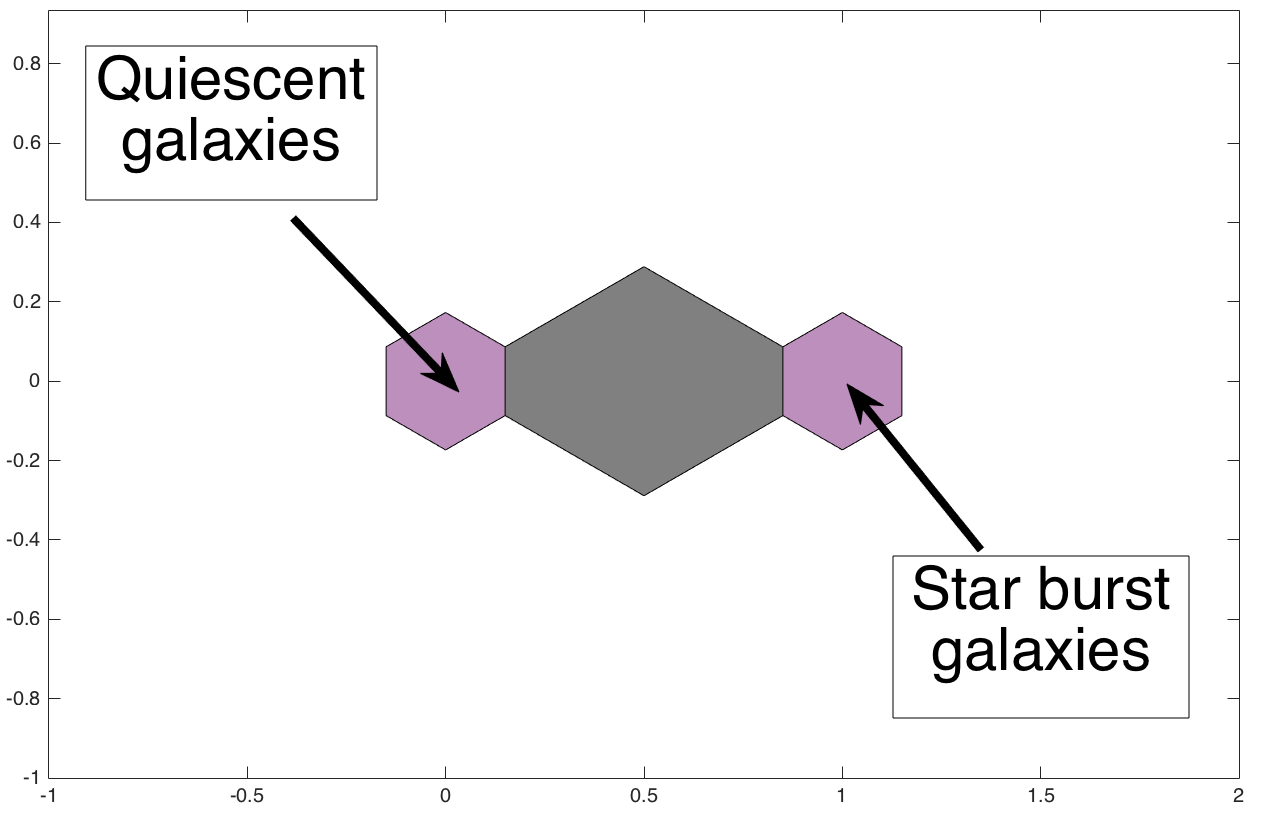
\includegraphics[width=\textwidth]{images0.01/1d/dist_1_by_2.png}
                \end{subfigure}
                \hfill
                \begin{subfigure}[b]{0.5\textwidth}
                     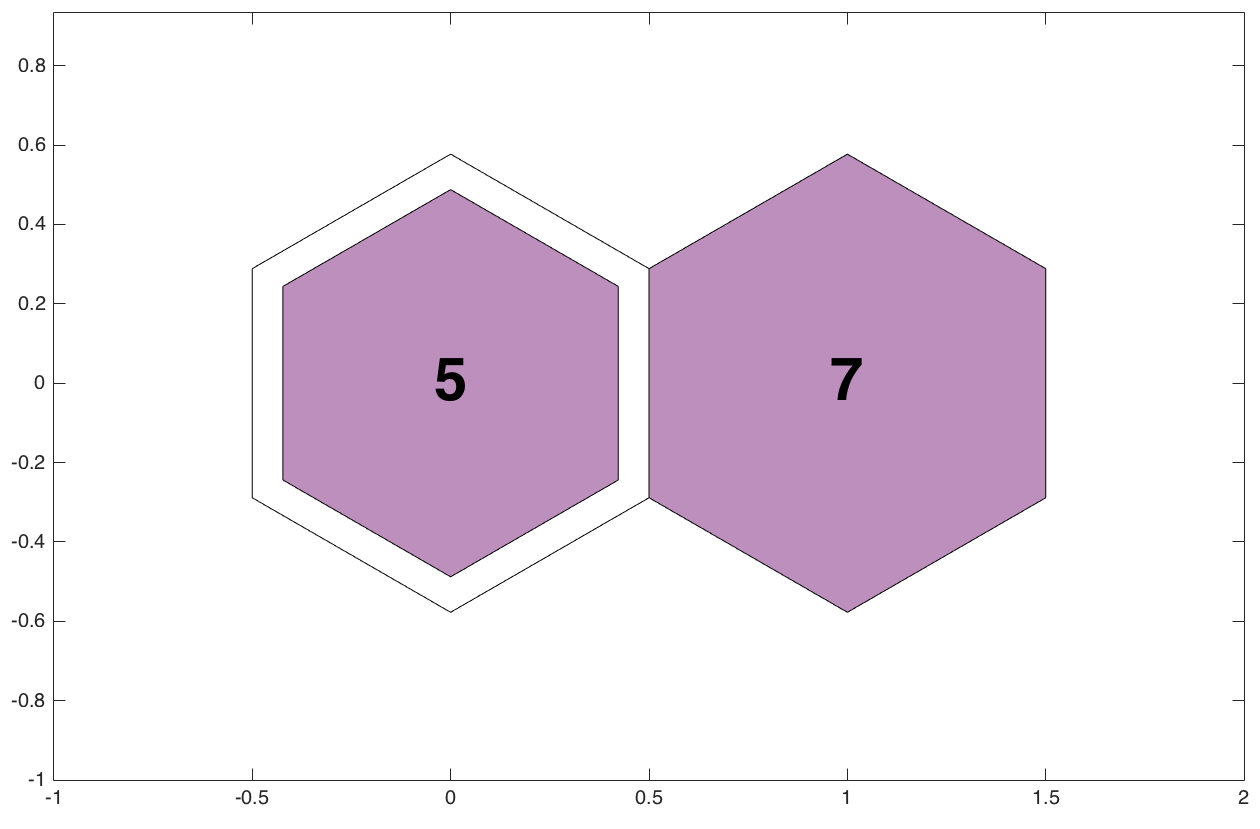
\includegraphics[width=\textwidth]{images0.01/1d/hit_t_1_by_2.png}
                \end{subfigure}
                \caption{Results of training network in $1\times2$~grid. Similar to Fig.~\ref{fig: sample} the upper plot is a distance map and the lower plot is a hit map. In this network, 5 of galaxies from K96 model, categorized as quiescent galaxies and the rest are starbursts. Because of their high emission lines, Sc galaxies moved towards the starburst ones.}
                 \label{fig: 1by2T}
            \end{figure}
        
        
            In the upper map in Fig.~\ref{fig: 1by2T}, the dark colour between two neurons indicates that the relative distance between these two groups are relatively high, and these two groups are distinguishable groups.
            In the lower part of Fig.~\ref{fig: 1by2T}, we see galaxies divided to two groups of 5 and 7.
            Although we know from K96 and T12 that 6 of the galaxies are quiescent and the other 6 are starbursts, the SOM results show 5 of the galaxies in one group and the other 7 in the second group.
            In this method, the Sc galaxies have been categorized as starburst galaxy due to the relatively higher amount of the disk stellar population relative to the bulge ones. 
            According to K96, Sc galaxies are considered as late Hubble type galaxies which have more flat SED compare to other quiescent galaxies. 
            

            Fig.~\ref{fig: 1by3T} shows the results of the training in a 1$\times$3 network.
            In these plots we forced the galaxies to categorize themselves in maximum 3 groups. 
            If the galaxies in Fig.~\ref{fig: 1by2T} were very similar to each other or were exactly the same, they still wanted to be divided into two groups and left the middle node empty. 
            However, in the lower part of Fig.~\ref{fig: 1by3T}, we can see that the middle node contains two galaxies.
            These two galaxies, which are separated from group of starburst galaxies in the lower part of Fig.~\ref{fig: 1by2T}, belong to SB5 and SB6 types.
            In the upper plot of Fig.~\ref{fig: 1by3T}, the colour between two right neurons is black and the colour between two left neurons is white. 
            The black colour indicates that the left neuron is completely different from the other two groups.
            While the white colour shows the two right neurons are very similar to one another. 
            
            Comparing Fig.~\ref{fig: 1by2T} with Fig.~\ref{fig: 1by3T} shows us that the starburst galaxies are divided into two groups. 
            Based on the colours between these two groups, we conclude that they are very similar groups; both groups are starburst galaxies and have strong emission lines.
            However, SB5 and SB6 types have the most internal extinctions.
            The high amount of extinction causes SED become more flat at shorter wavelength regions.
            The flatness in the UV part of the SED eventually makes these two types of galaxies become more similar to quiescent galaxies than other starburst ones.
            So in the networks, SB5 and SB6 types intend to move more towards the early type galaxies.
                
            \begin{figure}
                \begin{subfigure}[b]{0.5\textwidth}
                    \centering
                    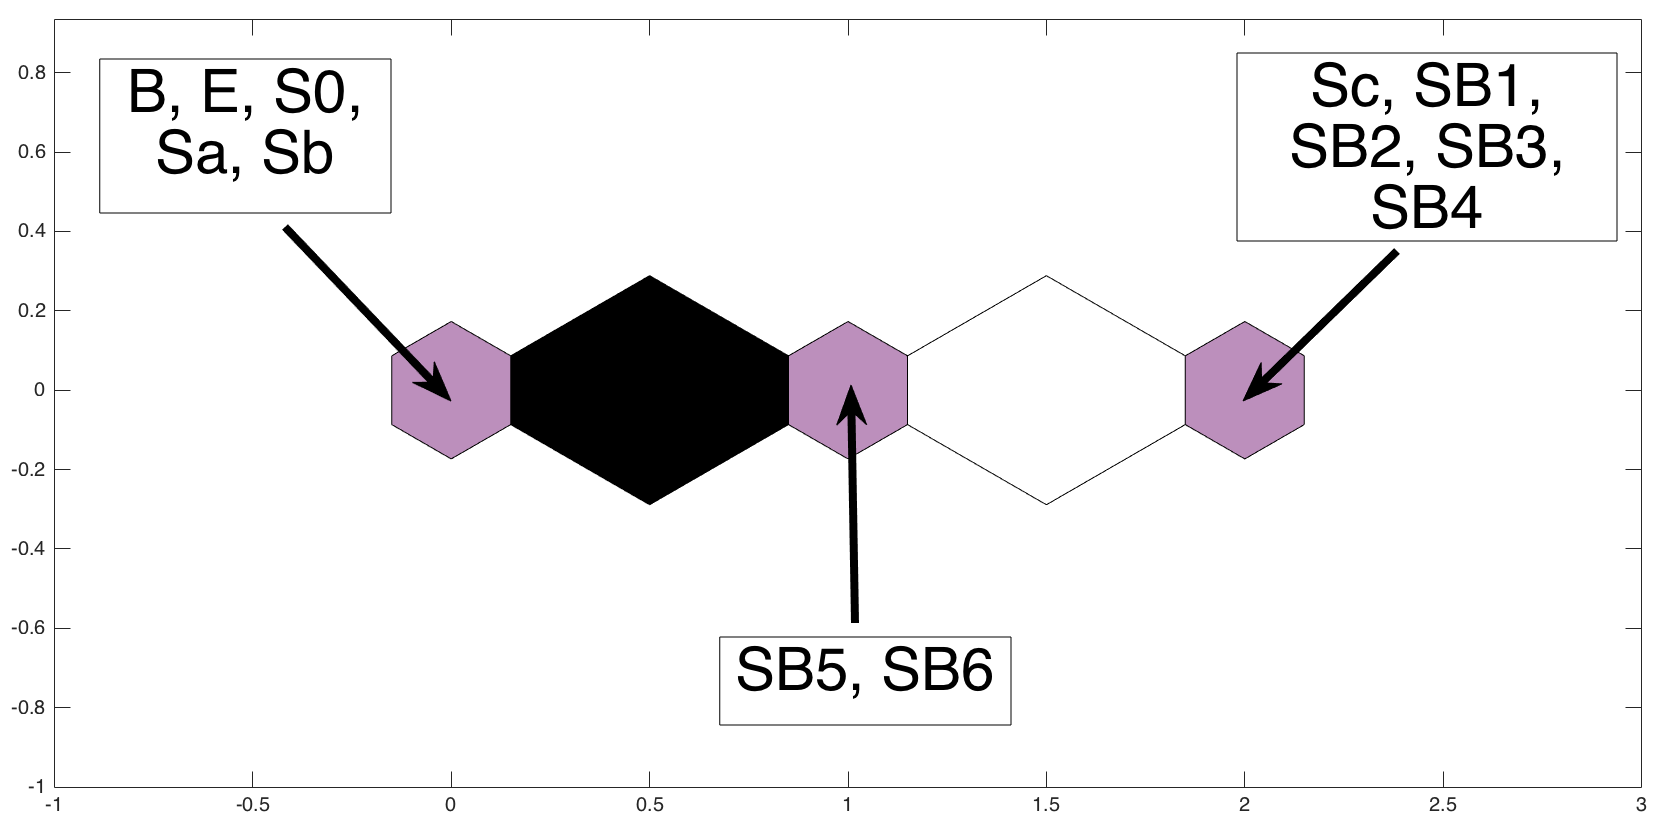
\includegraphics[width=\textwidth]{images0.01/1d/dist_1_by_3.png}
                \end{subfigure}
                \hfill
                \begin{subfigure}[b]{0.5\textwidth}
                     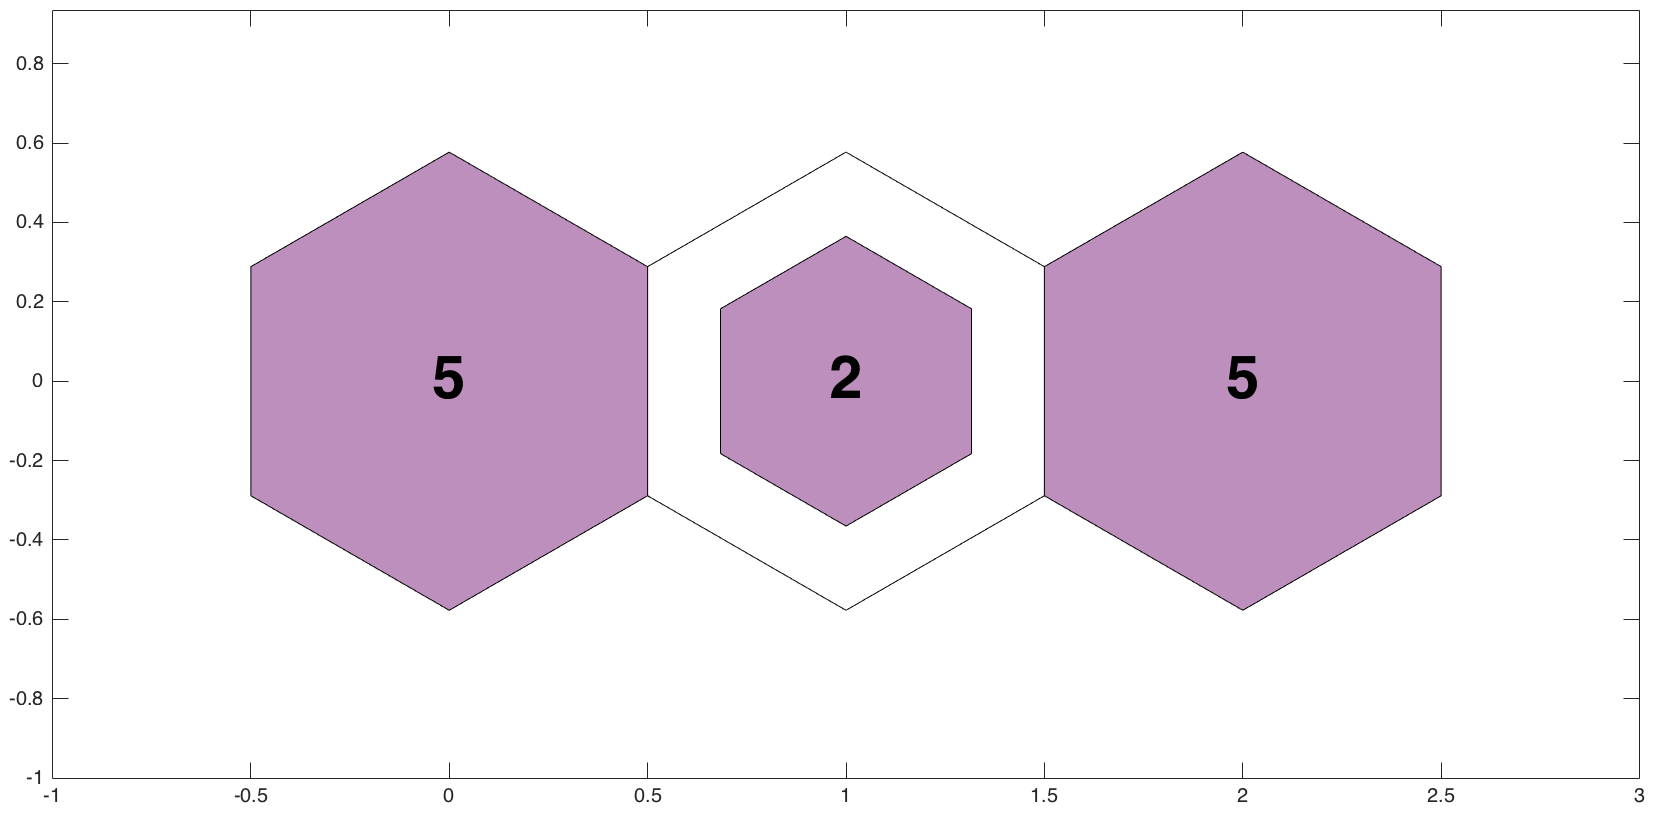
\includegraphics[width=\textwidth]{images0.01/1d/hit_t_1_by_3.png}
                \end{subfigure}
                \caption{The same as Fig.~\ref{fig: 1by2T} but this time the figure shows results of training network in $1\times3$~grid. In this network again, 5 of galaxies from K96 model, categorized as quiescent galaxies, and 7 as starbursts. However, this time 2 of galaxies (SB5, and SB6) are separated starbursts groups.}
                 \label{fig: 1by3T}
            \end{figure}
           
            We increased the size of maps gradually till the galaxies were divided into twelve groups (Figs.~\ref{fig: 1by4T} to ~\ref{fig: 1by20T} and ~\ref{fig: 1by22T}).
            Since there are more nodes in higher grid SOMs, the program pays more attention to small differences between each group.
            Higher the size of the maps means that even considering the smallest differences between galaxies.
            If the galaxies from K96 had completely different and distinct SED, SOM with size of $1\times12$ were expected to show 12 different groups of galaxies (1 at each node).
            However, in Fig.~\ref{fig: 1by12T}, we see that three of neurons contains two galaxies and three of them are empty, which shows there were no galaxy in K96 sample that can fill those neurons.
            In Fig.~\ref{fig: 1by12T} from left to right galaxies with types of B and E, SB3 and SB4, and SB1 and SB2, are the ones groups together. 
            The SB3 and SB4 grouping breaks when we increased the size of the network to $1\times15$~(Fig.~\ref{fig: 1by15T}).
            The SB1 and SB2 galaxies remained in the same neurons till we increased the size of map to $1\times20$~(Fig.~\ref{fig: 1by20T}), and the separation between galaxies B and E had not happened before the size of the SOM reached to $1\times22$~(Fig.~\ref{fig: 1by22T}).
        \begin{figure*}
            \begin{subfigure}[b]{\textwidth}
                \centering
                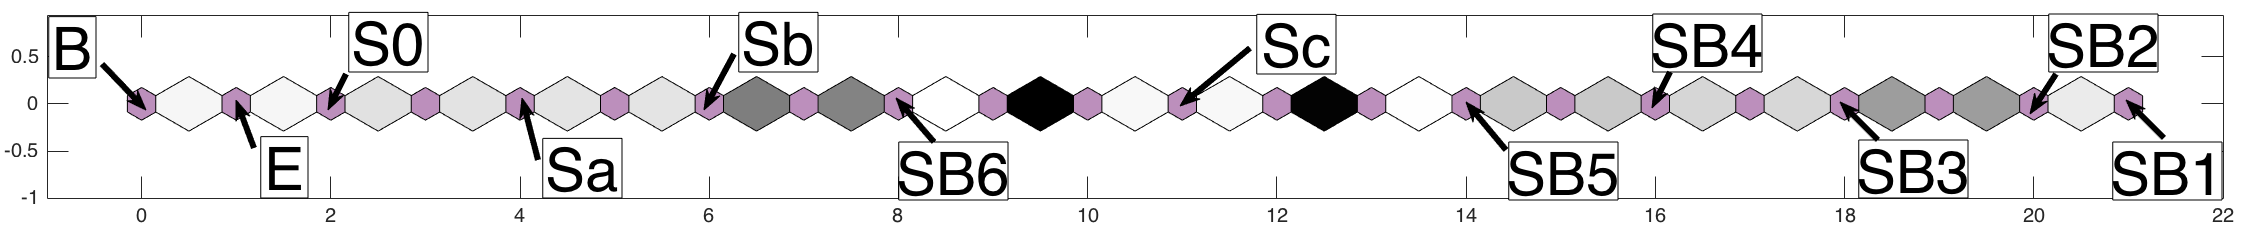
\includegraphics[width=\textwidth]{images0.01/1d/dist_1_by_22.png}
            %\caption{$1\times22$ weight map}
             %\label{fig: 1by22T}
            \end{subfigure}
            \hfill
            \begin{subfigure}[b]{\textwidth}
                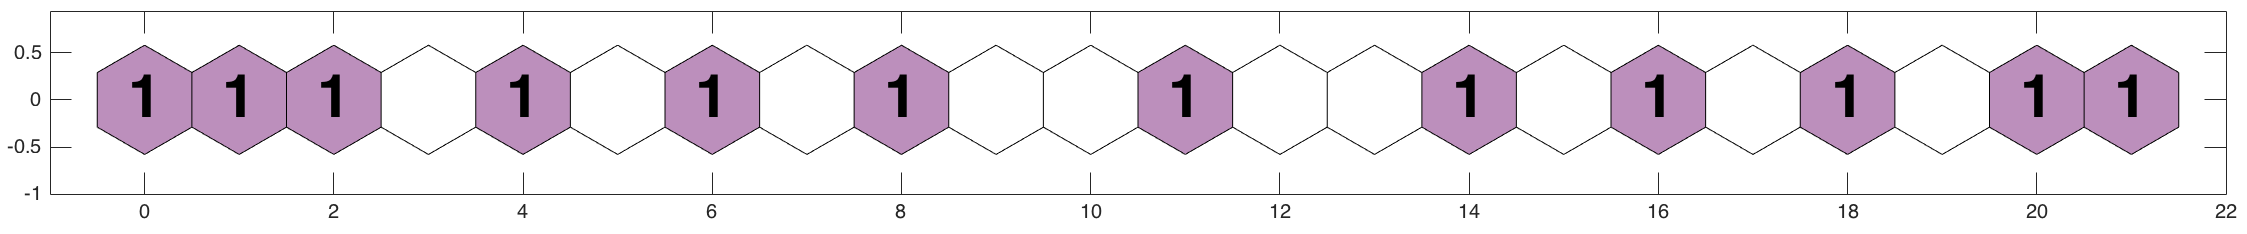
\includegraphics[width=\textwidth]{images0.01/1d/hit_t_1_by_22.png}
             %\caption{$1\times22$ hits map}
             %\label{fig: 1by22Thits}
            \end{subfigure}
            \caption{The same as Fig.~\ref{fig: 1by2T} but this time the figure shows results of training network in $1\times22$~grid.}
            \label{fig: 1by22T}
        \end{figure*} %PB160427: this figure looks really great! Very easy to understand.
    
            In Fig.~\ref{fig: 1by22T}, in lower plot we can see twelve different groups. 
            In upper plot 5 groups are in the left side neurons, and there are two dark grey colours between them and then the rest of the galaxies. 
            It shows that although we separated the galaxies in twelve groups, but they are still divided in two main groups.
            The closest occupied neurons in the starburst side of the SOM, belongs to the SB6 type. 
            This type of the galaxies has the most extinction and its SED has similarity to early type galaxies more than other starburst types. 
            
            The fact that the galaxies had to have 22 different neurons till be divided into 12 groups, shows that the difference between SB1 and SB2, and B and E galaxies are very small.
            %These small differences might be very small.
            Therefore, they intend to stay in the same group till the network become big enough to make attention to the smallest particularity.
           
        \subsubsection{ CLASSIFYING SAMPLE OF GALAXIES}
         \label{sec: 1Dv}
            We used each network that we trained in Sec.~\ref{sec: 1Dt}, to classifying the sample 142 galaxies from T12.
            Upper plot in Fig.~\ref{fig: 1by2V} shows the result of the classifying of the T12 galaxies using the $1\times2$~network from Fig.~\ref{fig: 1by2T}.
            It shows that 80 of the galaxies have SEDs similar to the early type galaxies and the SEDs of the rest of them are similar to starburst galaxies.
            The lower plot shows the average SED of the galaxies in each node. 
            The left plot shows the average SED of 80 galaxies that classify as an early type galaxies. 
            These galaxies are similar to the ones in the left node in the upper plot in Fig.~\ref{fig: 1by2T}.
            The plots clearly show the 4000\AA~break in the SEDs, which is one of the signatures of the early type galaxies.
            The strong emission lines in that figure could be from the galaxies with similar SED to Sa galaxies but with more strong emission lines.
            The right plot in the lower part of Fig.~\ref{fig: 1by2V} shows strong emission lines and high emissions in the lower wavelengths, which are the signs of the strong star formation in the galaxies. 
            \begin{figure}
                \begin{subfigure}[b]{0.5\textwidth}
                    \centering
                    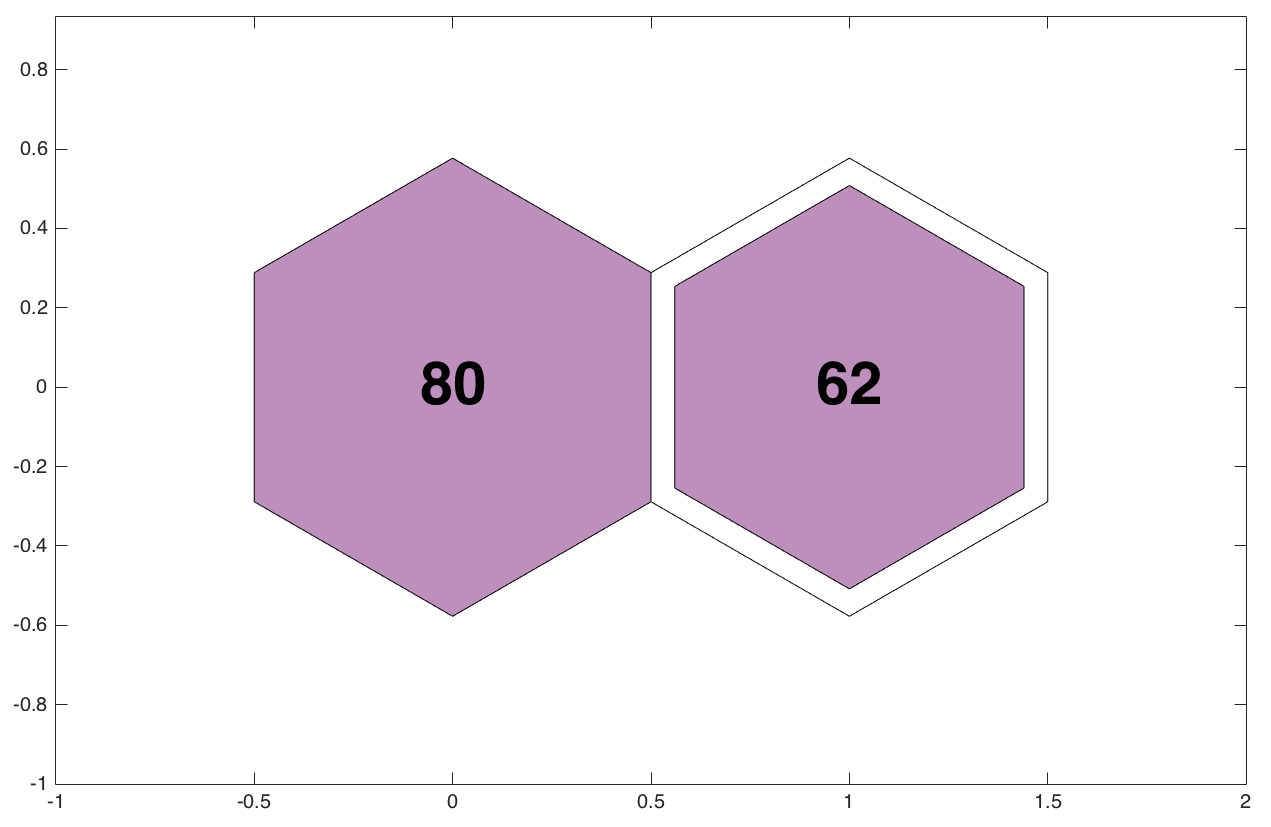
\includegraphics[width=\textwidth]{images0.01/1d/hit_v_1_by_2.png}
                    %\caption{$1\times2$ weight map}
                     %\label{fig: 1by3T}
                \end{subfigure}
                \hfill
                \begin{subfigure}[b]{0.5\textwidth}
                     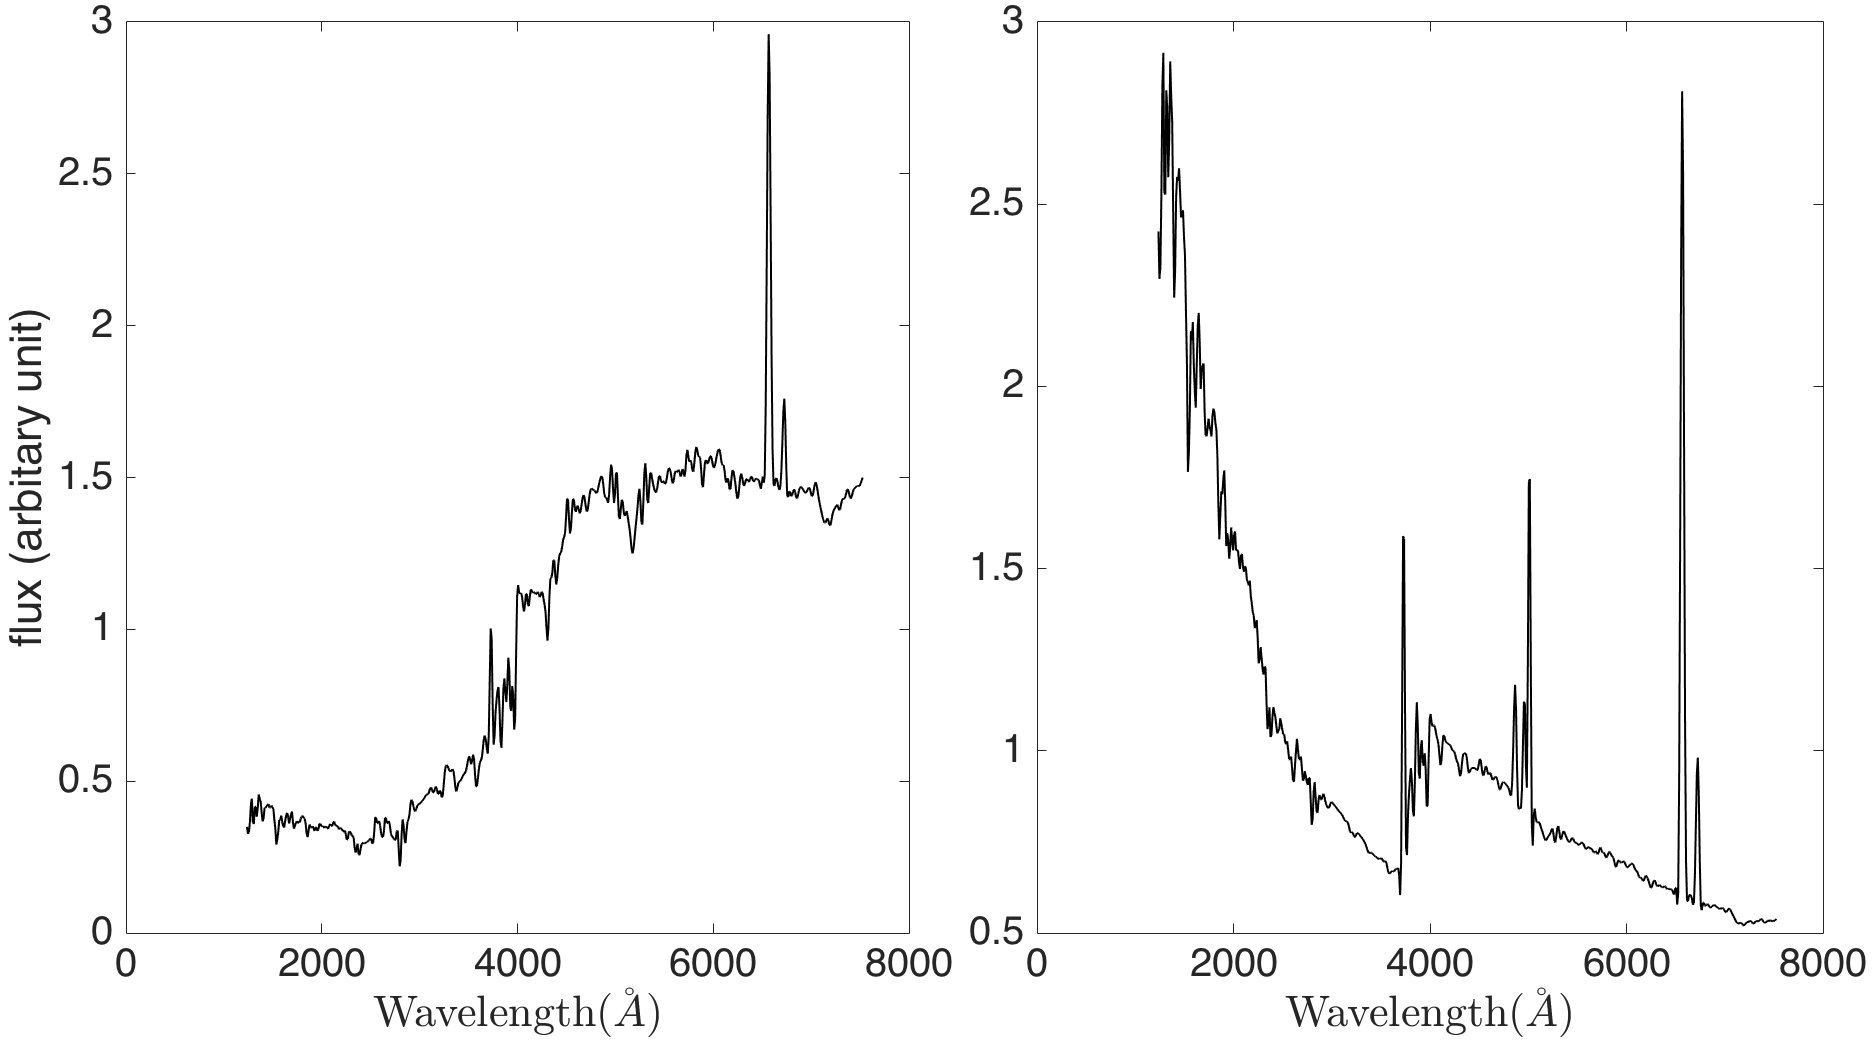
\includegraphics[width=\textwidth]{images0.01/1d/SED_total1by2.png}
                     %\caption{$1\times2$ hits map}
                     %\label{fig: 1by3Thits}
                \end{subfigure}
                \caption{Classifying galaxies from T12, based on their SEDs using $1\times2$~networks that were trained from 12 galaxies in Fig.~\ref{fig: 1by2T}. Up: the same as other hit maps, numbers in each node represents the number of galaxies that belong to that group. In this case 80 means that 80 of the 142 galaxies classify as the early type groups while the 62 of the 142 galaxies categorize to the starburst galaxies. Down: Average SED of the SEDs of the galaxies in each group. The left plot shows the average SED of the 80 galaxies (early type ones), and the right plot shows the average SED of the SEDs of 62 galaxies (the starburst ones).}
                \label{fig: 1by2V}
            \end{figure}            
            Since in this network galaxies forced to be divided into maximum two groups, for any SED between these two groups the SOM must decide that each galaxy belongs to which group based on strongest features of its SED.
            The galaxies with a weak 4000\AA~break but strong emission lines and increase of the flux in the lower wavelengths categorized as starbursts while galaxies with strong 4000\AA~break, but no emission lines categorized as the early type.
            Increasing the size of the SOM helps to solve the problem of the galaxies which have features of both groups.
            
             Fig.~\ref{fig: 1by3V} represents the result of the classifying the SED of the galaxies using the $1\times3$~network (from Fig.~\ref{fig: 1by2T}). 
             In the upper plot of this figure we can see 66 of the galaxies belongs to the early type group, and 47 belong to starburst galaxies. 
             29 of the galaxies are more similar to starburst ones, but not with all of their features. 
             These groups of galaxies have strong emission lines and rising flux towards the ultraviolet, but they also have a strong 4000\AA~break, which makes them to move towards the early type galaxies (middle plot in the lower part of Fig.~\ref{fig: 1by2V}).

            \begin{figure}
                \begin{subfigure}[b]{0.5\textwidth}
                    \centering
                    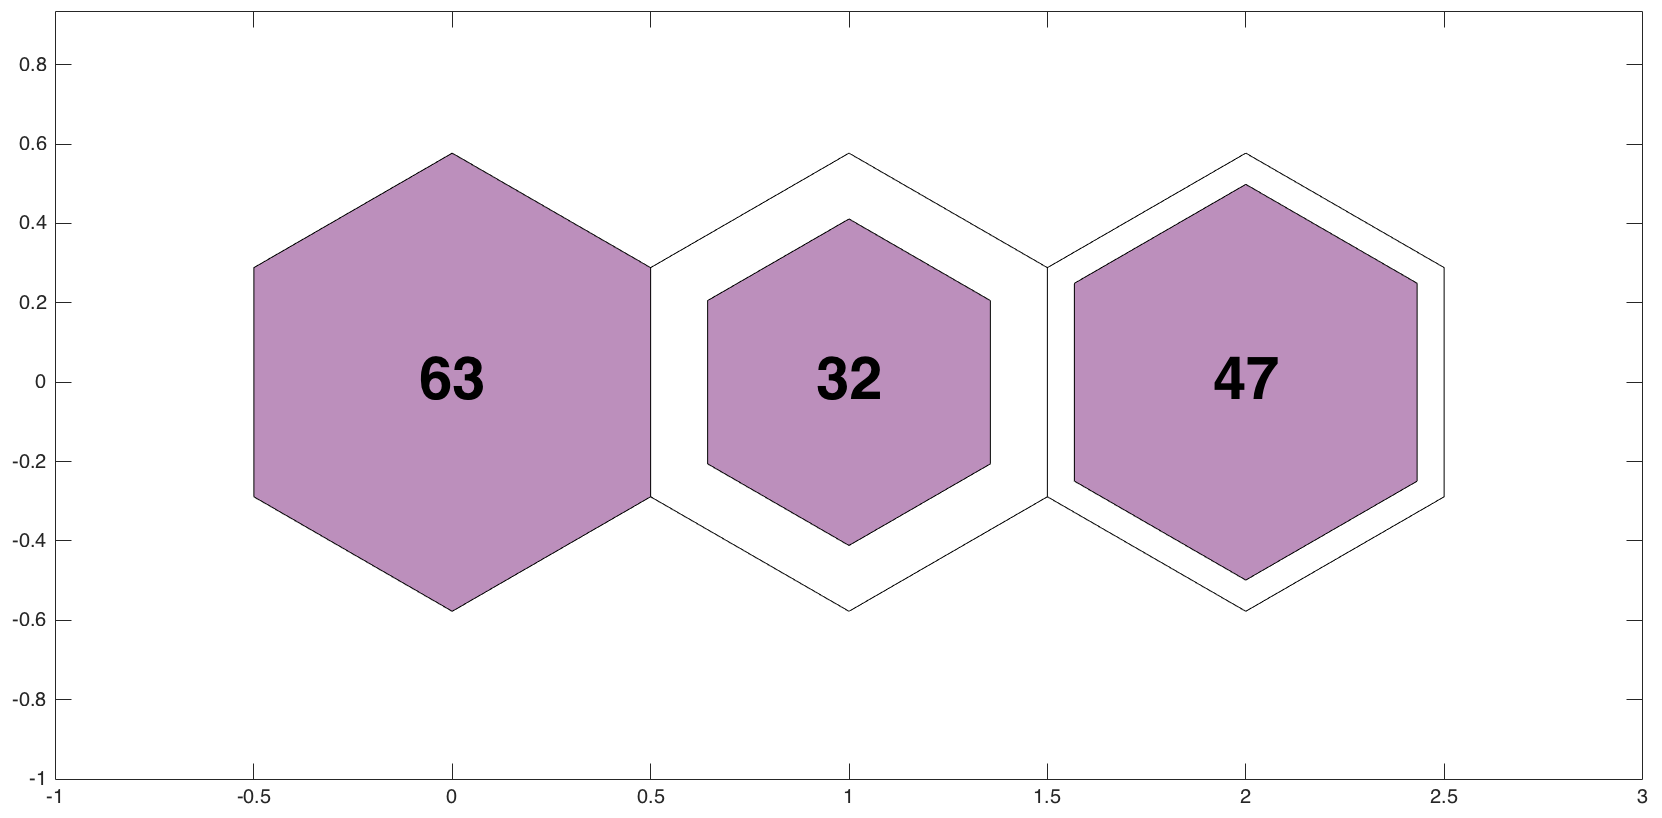
\includegraphics[width=\textwidth]{images0.01/1d/hit_v_1_by_3.png}
                    %\caption{$1\times2$ weight map}
                     %\label{fig: 1by3T}
                \end{subfigure}
                \hfill
                \begin{subfigure}[b]{0.5\textwidth}
                     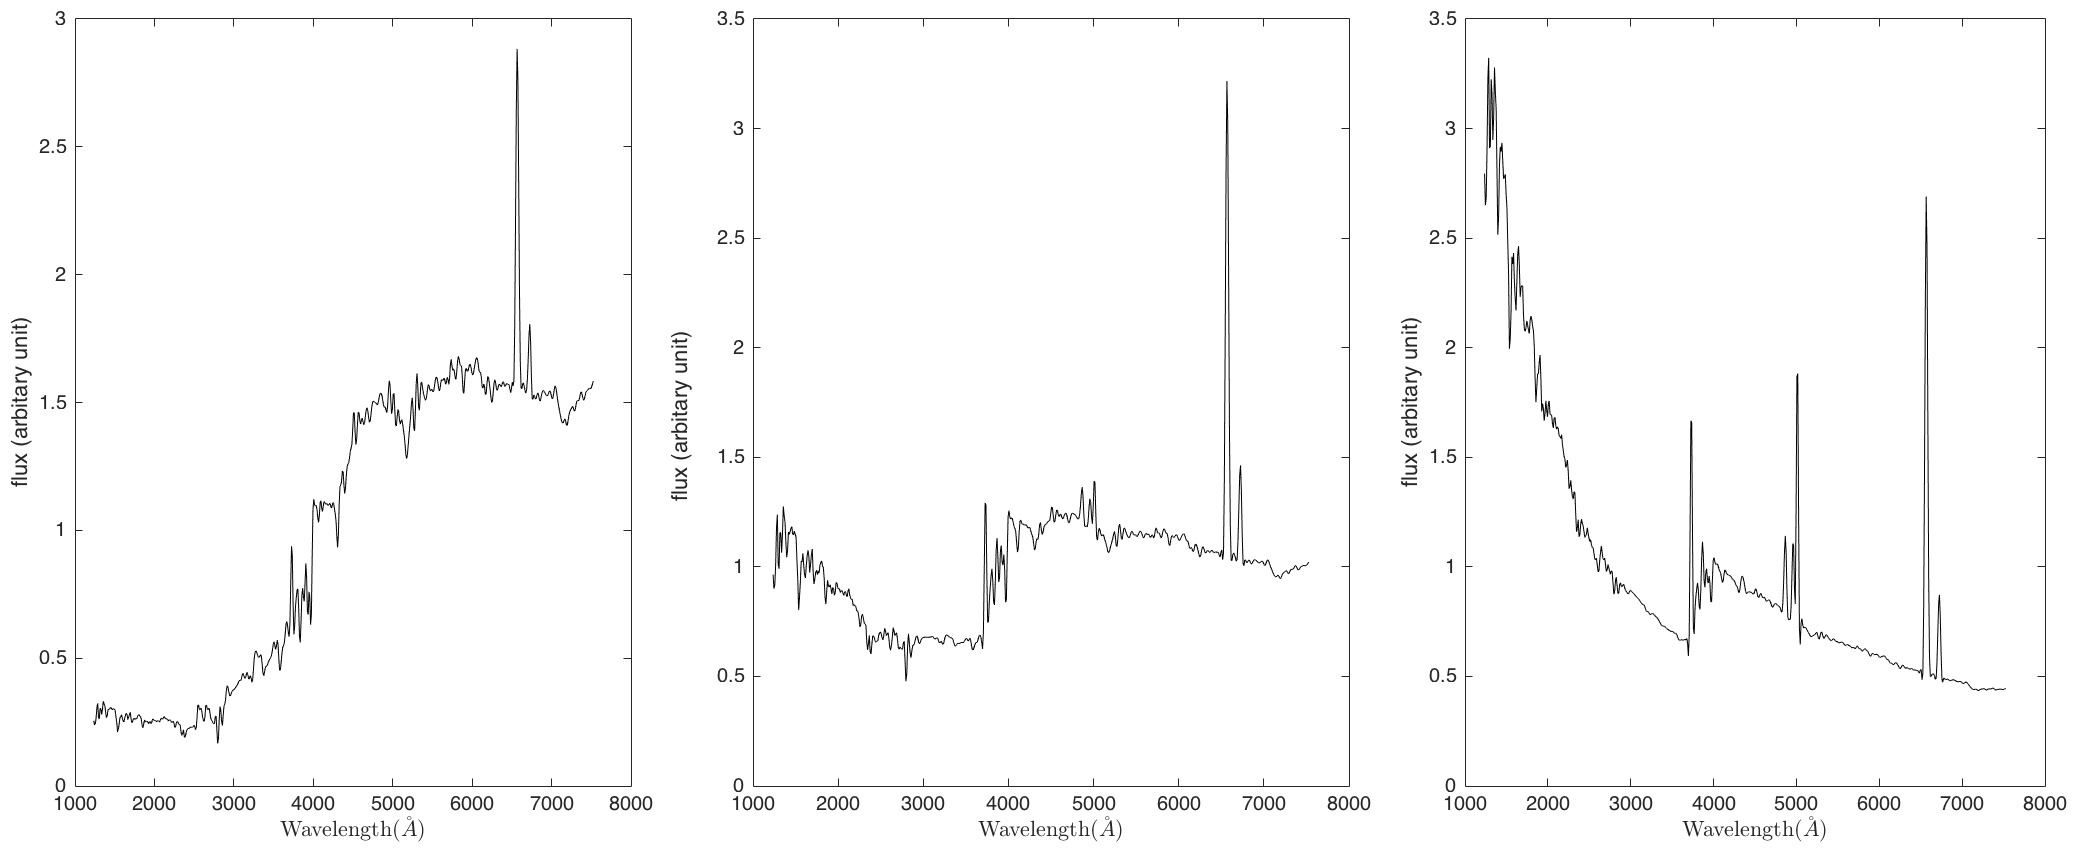
\includegraphics[width=\textwidth]{images0.01/1d/SED_total1by3.png}
                     %\caption{$1\times2$ hits map}
                     %\label{fig: 1by3Thits}
                \end{subfigure}
                \caption{Same as Fig.~\ref{fig: 1by2V}, but in this figure, we used network with size of $1\times3$ (Fig.~\ref{fig: 1by3T}) to classify the sample galaxies.}
                \label{fig: 1by3V}
            \end{figure}       
            
            In Fig.~\ref{fig: 1by22V}, we used the $1\times22$~network to classify the sample galaxies.
            As mentioned in the Sec.~\ref{sec: 1Dt}, this network size is the first size that we could see the K96 galaxies separated in 12 different neurons.
            B and E or SB1 and SB2 galaxies were too similar to SOM can recognize them as two separate groups.
            The same as Figs.~\ref{fig: 1by2V} and ~\ref{fig: 1by3V}, upper plot of Fig.~\ref{fig: 1by22V} shows how many of galaxies from the 142 galaxies, moved to each neuron in the $1\times22$ SOM.
            \begin{figure*}
                \begin{subfigure}[b]{0.9\textwidth}
                    \centering
                    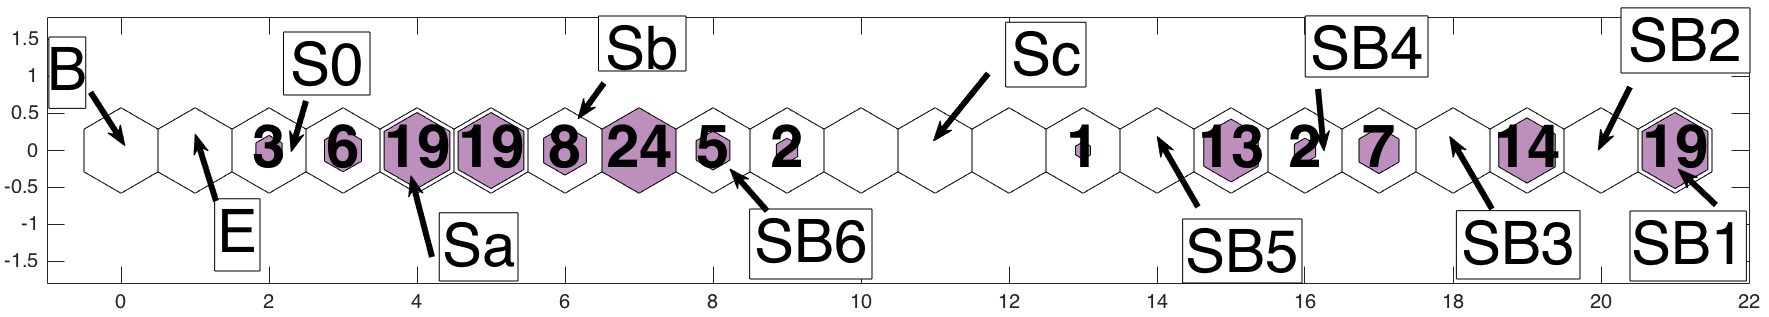
\includegraphics[width=\textwidth]{images0.01/1d/hit_v_1_by_22_n.png}
                    %\caption{$1\times2$ weight map}
                     %\label{fig: 1by3T}
                \end{subfigure}
                \hfill
                \begin{subfigure}[b]{0.9\textwidth}
                     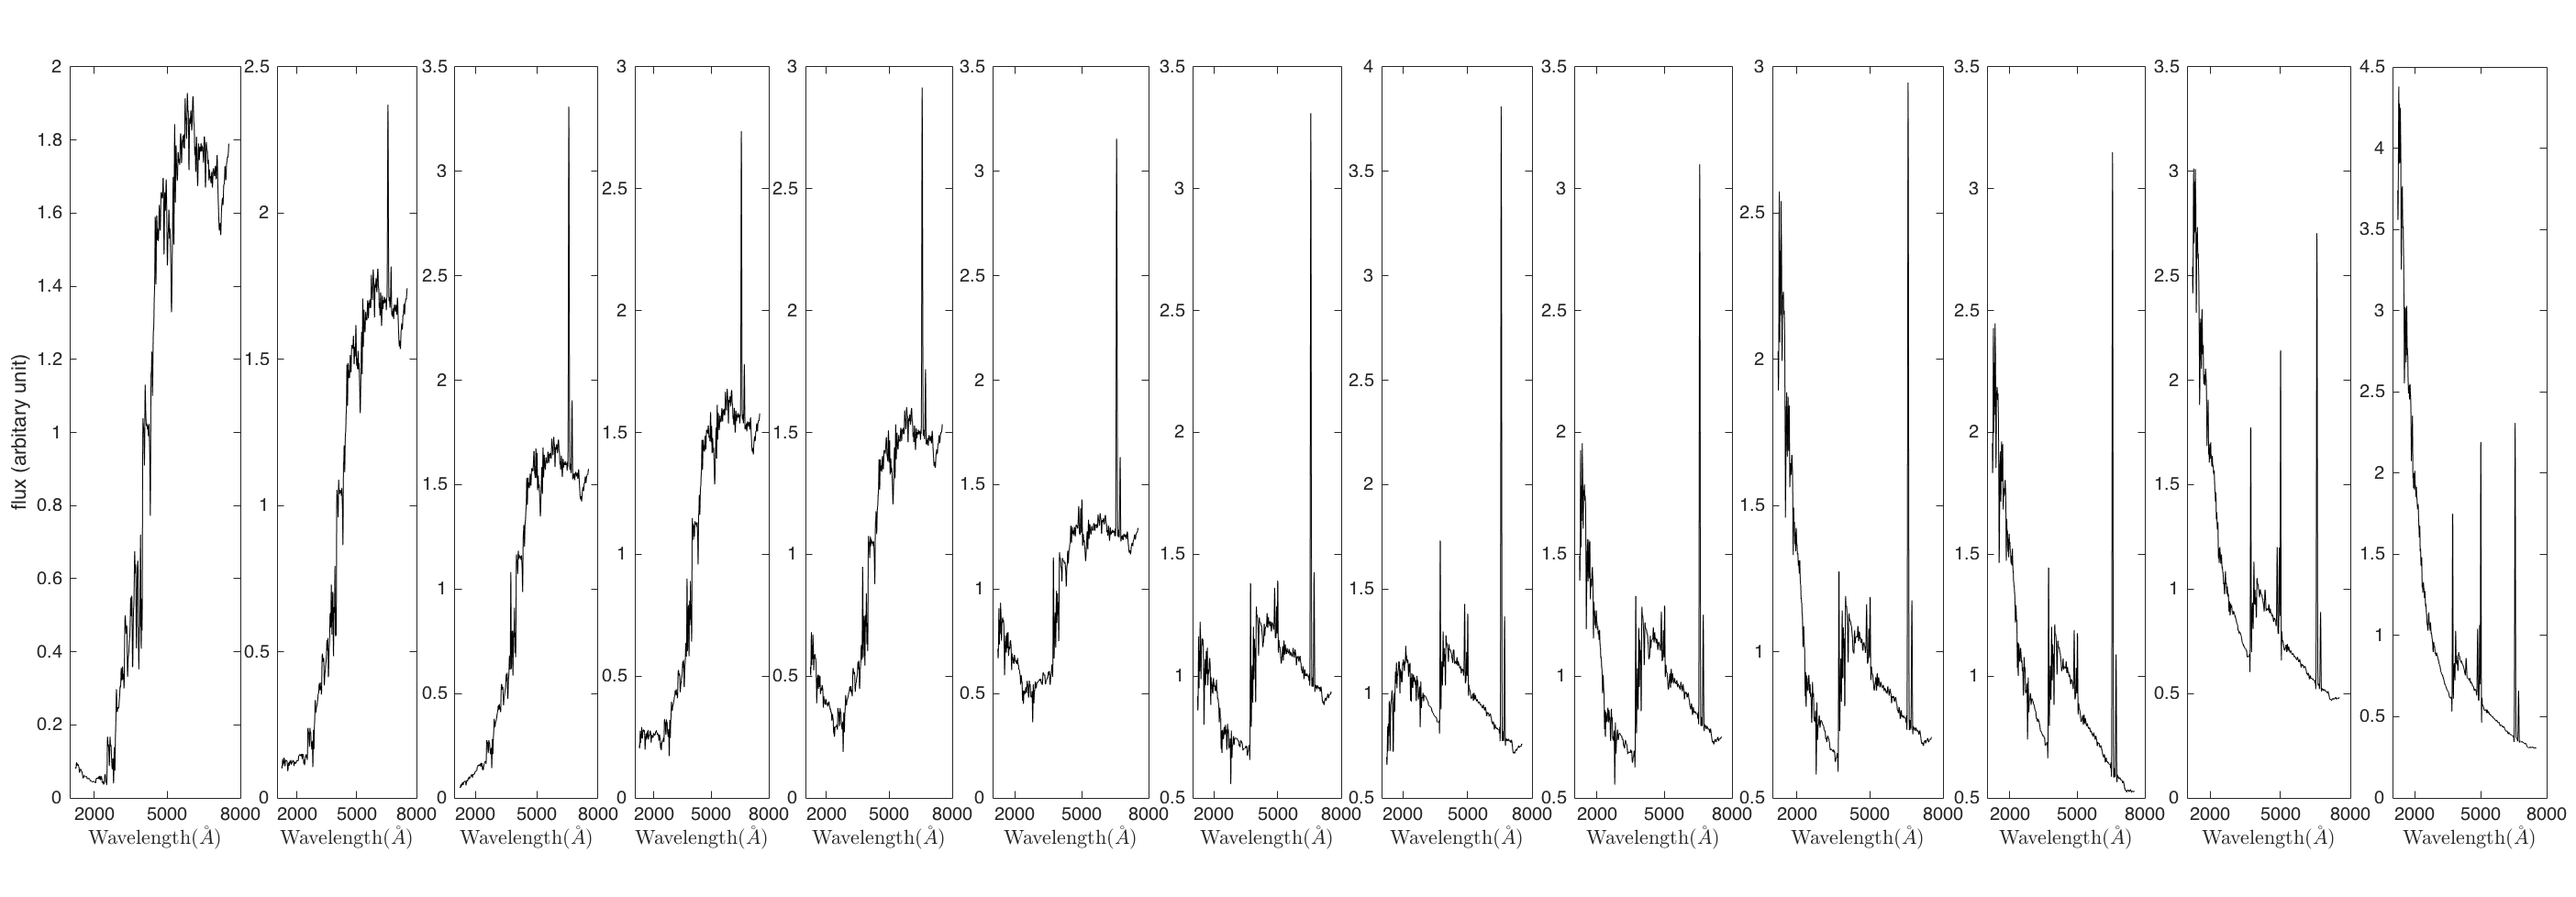
\includegraphics[width=\textwidth]{images0.01/1d/SED_total1by22.png}
                     %\caption{$1\times2$ hits map}
                     %\label{fig: 1by3Thits}
                \end{subfigure}
                \caption{Same as Fig.~\ref{fig: 1by2V}, but in this figure, we used a network with size of $1\times22$ (Fig.~\ref{fig: 1by22T}) to classify the sample galaxies. In the average SED of each neuron, we can clearly see the changes from early type galaxies in the starburst ones. 4000\AA~ break reduces from left to right and emission lines increase.}
                \label{fig: 1by22V}
            \end{figure*}
            The lower plot of the figure represents the average SED of the galaxies in each neuron.
            However, this time, since galaxies had more space to separate some of the neurons left empty. 
            Thus, instead of having 22 average SED plots in the lower part of Fig.~\ref{fig: 1by22V}, we have 12 SEDs.
            
            By comparing the upper part of Fig.~\ref{fig: 1by22V} with the lower part of Fig.~\ref{fig: 1by22T}, we can see that the occupied neurons are not necessarily the same.
            If a group of T12 galaxies fills the same neurons as the K96 galaxies, we can conclude that these galaxies have SEDs very similar to the SED of one of K96 galaxies.
            Whereas, we can conclude that a group of galaxies has properties between the two groups if they fill a neuron which is empty and is placed between two categories of galaxies in Fig.~\ref{fig: 1by22T}.
            However, the colours between these neurons in the upper side of Fig.~\ref{fig: 1by22T}, establishes that those galaxies are more similar to which group. 
            
            In the first two neurons of the upper plot in Fig.~\ref{fig: 1by22V}, there is no galaxy, while in galaxies B and E are in the same neurons in the trained network.
            So we can conclude that there is no galaxy with similar specification of type B or E in the T12 sample.
            There are 3 galaxies in the third neuron, which shows these 3 galaxies are very much similar to the S0 type. 
            18 of the galaxies are on the fifth neurons and similar to the Sa type of the galaxies, while the 7 galaxies in the fourth neurons have SEDs similar to both S0 and Sa galaxies.
            There is one Sb type galaxy and 15 galaxies with SED similar to both Sa and Sb type galaxies.
            The following two neurons (eighth and ninth neurons from the left) are on the edge of the early type and starburst galaxies.
            In the upper plot in the  Fig.~\ref{fig: 1by22T}, the colour between these two neurons are black, which indicates that the weights between these two are really different from each other.
            Therefore, 24 galaxies in the eighth neurons have similar SEDs to Sb type galaxies and SEDs of the 14 galaxies in the ninth neurons are similar to the SB6 galaxies.
            The far right of the network, galaxies with SED comparable to type SB1 and SB2.
            
            In general, 56 galaxies correspond exactly to K96 types and the other 86 are in between of the initial 12 suggestions.
            As T12 mentioned, part of the reason we could not classify all the galaxies using the K96 model is that the model were constructed from co-adding 12 spectra of the 70 galaxies.
            In this small sample, it is quite possible that the best SEDs do not match any model, perfectly and the original classifications have high uncertainty.
            
            On the other hand, all the other methods (i.e. $\chi^2$ fitting, trained neural network) of matching SEDs limit themselves to models, and if they could not find the best match, report the results as uncertain ones.
            However, with SOM, galaxies have this freedom to be categorized in the intermediate groups.
            Therefore, if the SED of galaxies do not match completely with any of the model SEDs in Fig.~\ref{fig: k96}, they can be categorized as a SED with similarity to two or more of the groups.

                        
        
        
        \subsubsection{1D NETWORKS results and Properties of clustered galaxies}
        
        In order to check whether our conclusions in Sec.~\ref{sec: 1Dv}~is meaningful and correct, in this section we are going to show the relations between properties of the galaxies in each neuron.
        
        \begin{figure}
            \centering
            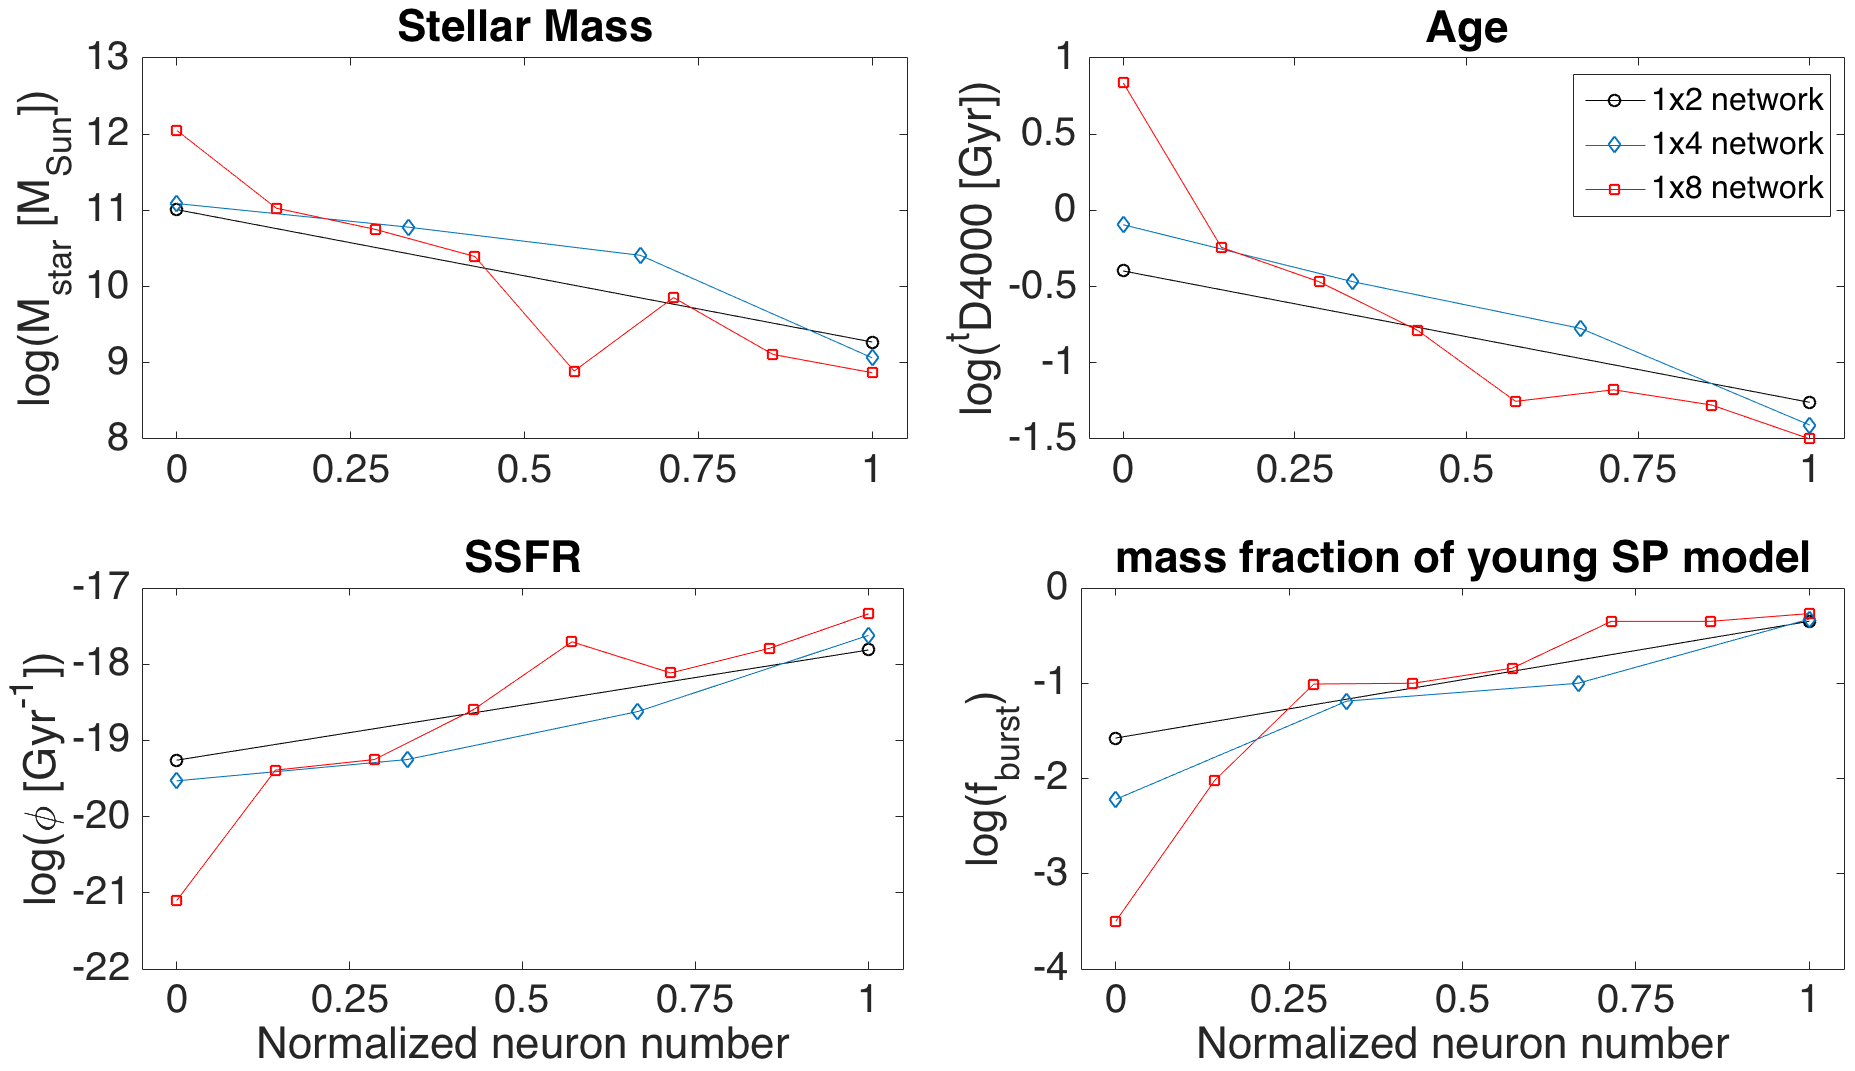
\includegraphics[width=0.5\textwidth]{images0.01/1d/props5.png}
            \caption{Comparing the median of four propertied of galaxies in each nod in $1\times2$ (balck circles), $1\times4$ (blue diamond), and $1\times8$ (red triangles) networks.}
            \label{fig: props}
        \end{figure}
       
        Fig.~\ref{fig: props} shows the results of the median of stellar mass, age, specific star formation rate (sSFR; star formation rate per stellar mass), and $f_\mathrm{burst}$ of the galaxies in each neuron in $1\times2$, $1\times4$, and $1\times8$ networks.
        In all the plots horizontal axis shows the number of the neurons divided by the size of the network, and vertical axis shows one of the mentioned properties.
        
        In Fig.~\ref{fig: props}, from early type galaxies to starburst ones, stellar mass and age decreases while sSFR and $f_\mathrm{burst}$ increases, in all three lines. 
       % These trends are another evidence that this method is working and can be used to categorize galaxies based on their SEDs or even their physical properties. 
        Considering results from Fig.~\ref{fig: props}, we can clearly see that separating galaxies based on SED types also leads to a separation in properties derived (via {\em CIGALE}) from the SEDs.
    
        N09 used various models to derive galaxies' properties.
        Through these models, some of the properties are already known to be correlated with each others, i.e. stellar mass and star formation rate.
        They, however, studied other relations between properties, that didn't have any direct correlation in the models, in a sample of SINGS galaxies. %%eHMM I will change the previous sentence! It doesn't read well
        They found a tight correlation between sSFR and t$_{\rm {D4000}}$, which suggested that younger stellar population correlate with high SFR.
        They also found the correlation between stellar mass and SFR, and stellar mass and t$_{\rm {D4000}}$.
        Since in {\em CIGALE} code, stellar mass is a free parameter, N09 argued that any stellar mass related correlation must be astrophysically meaningful. 
        They also studied relations between the attenuation at 1500 \AA~(A$_{\rm {FUV}}$) and sSFR, age, and stellar mass and did not find any correlation.
        T12 replicated the upper plots in Fig.~\ref{fig: props_vs_props}, and found a tighter correlation than N09 results. 
        
               \begin{figure*}
        \begin{subfigure}[b]{0.3\textwidth}
            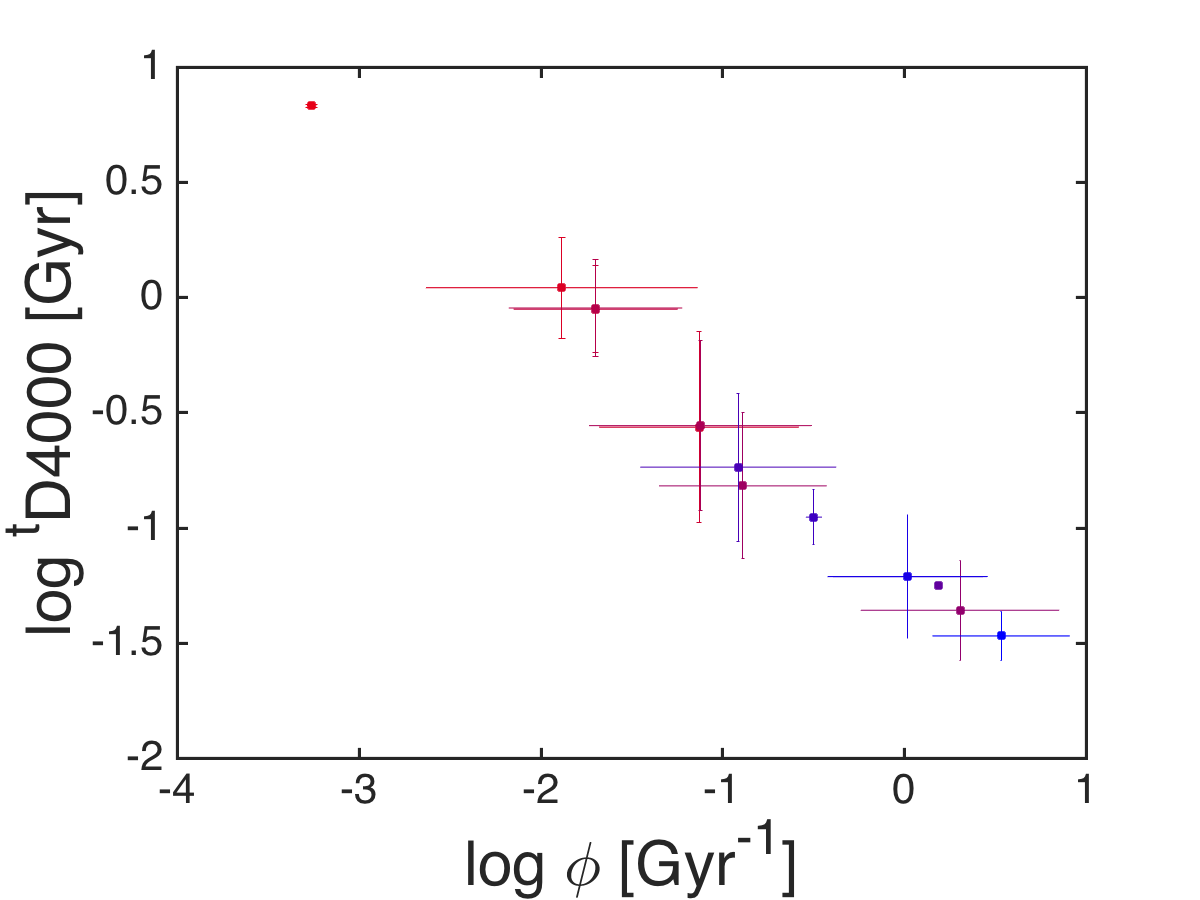
\includegraphics[width=\textwidth]{images0.01/1d/f1.png}
        \end{subfigure}
        \hfill
        \begin{subfigure}[b]{0.3\textwidth}
            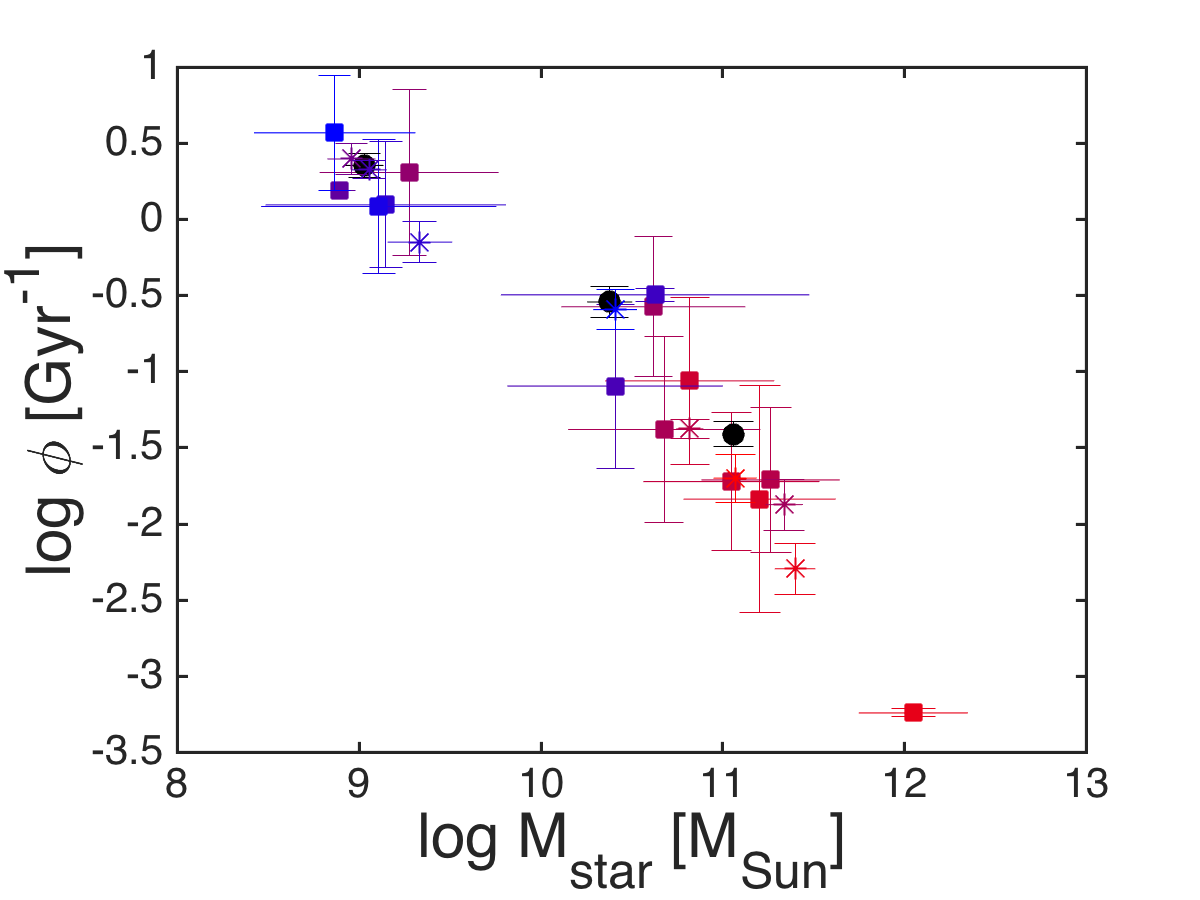
\includegraphics[width=\textwidth]{images0.01/1d/f2.png}
        \end{subfigure}
        \hfill
        \begin{subfigure}[b]{0.3\textwidth}
            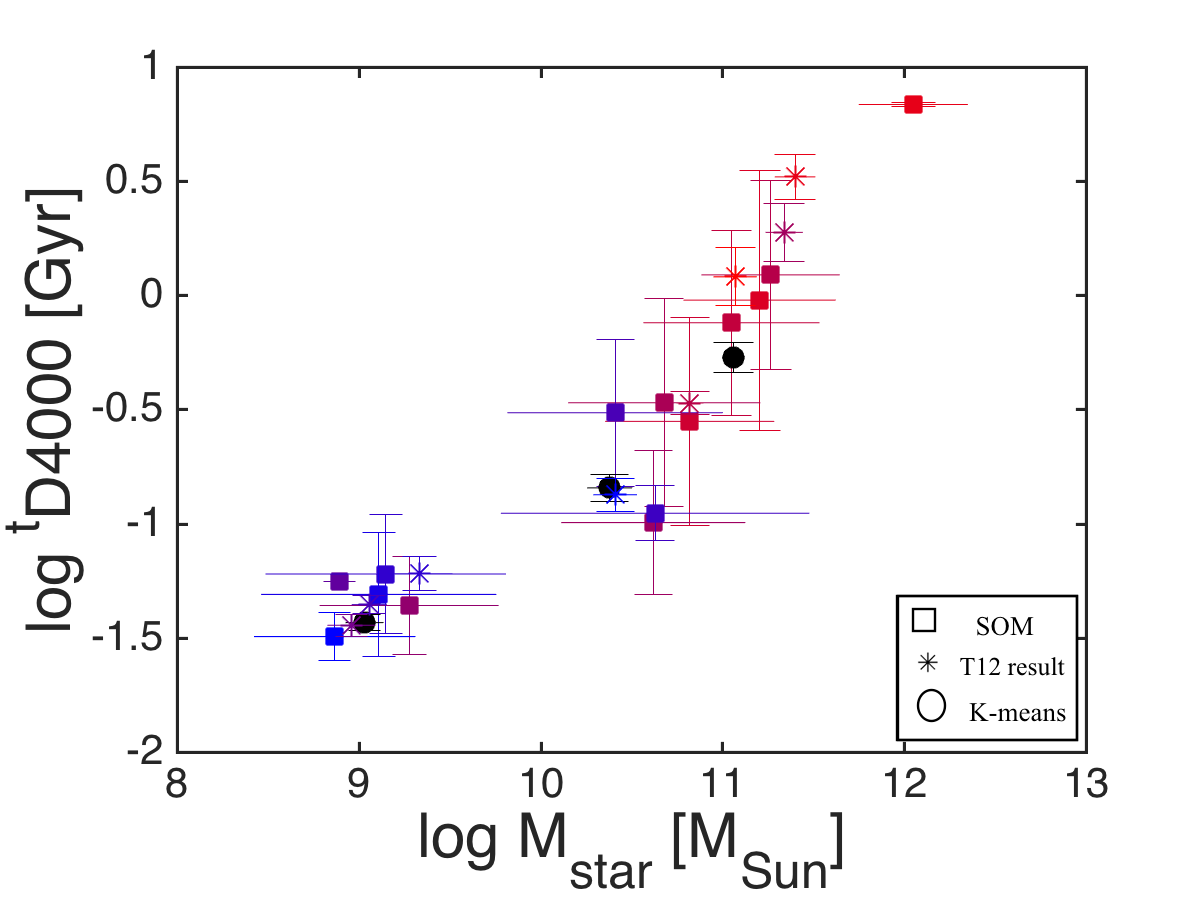
\includegraphics[width=\textwidth]{images0.01/1d/f3.png}
        \end{subfigure}
        \hfill
        \begin{subfigure}[b]{0.3\textwidth}
            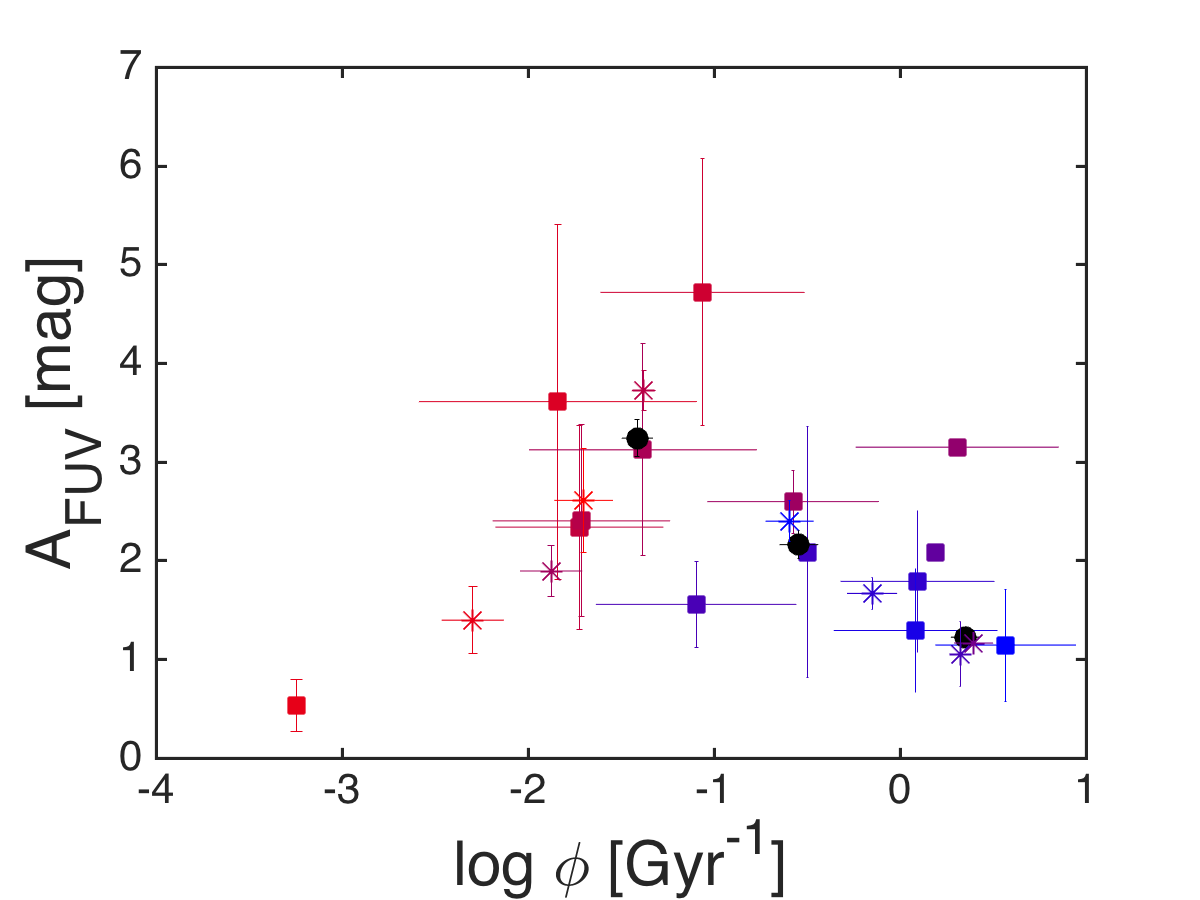
\includegraphics[width=\textwidth]{images0.01/1d/f4.png}
        \end{subfigure}
        \hfill
        \begin{subfigure}[b]{0.3\textwidth}
            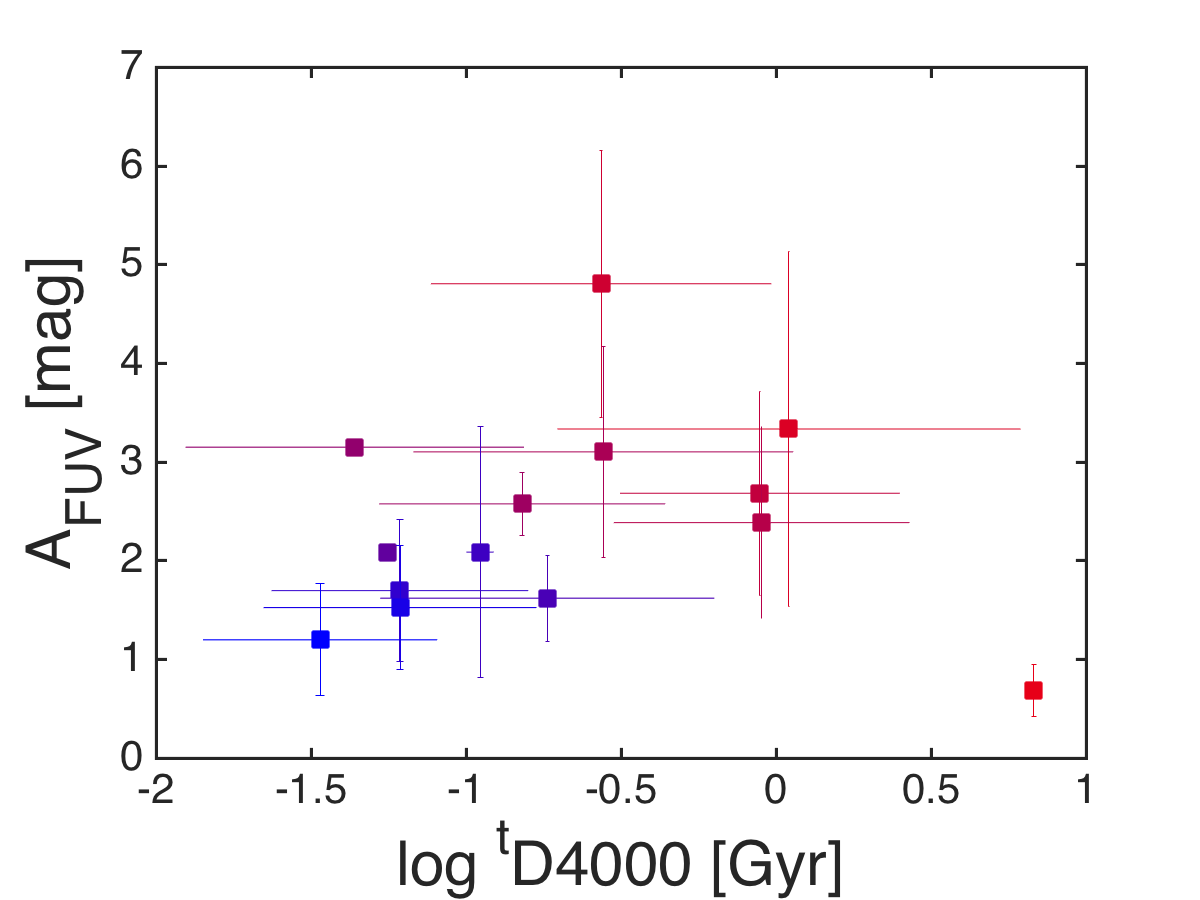
\includegraphics[width=\textwidth]{images0.01/1d/f5.png}
        \end{subfigure}
       \hfill
        \begin{subfigure}[b]{0.3\textwidth}
            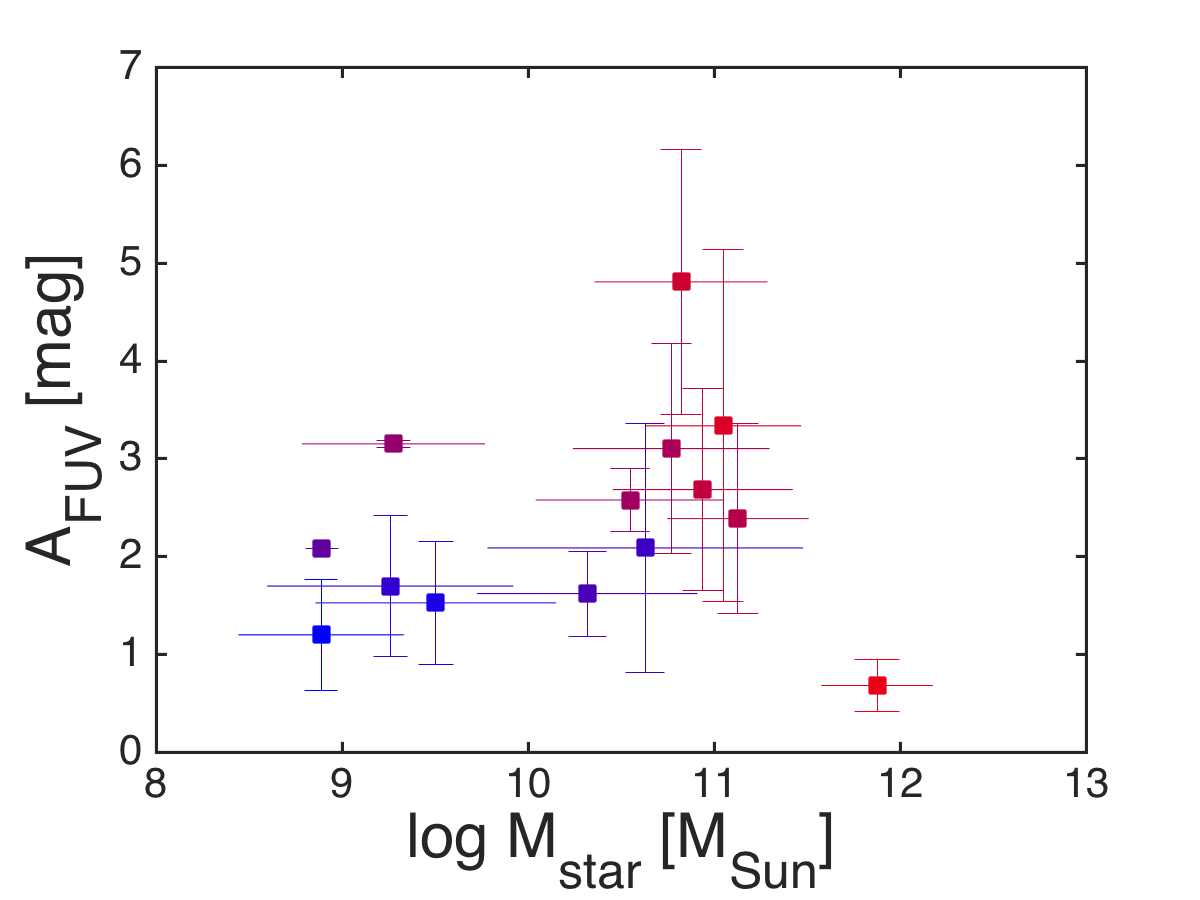
\includegraphics[width=\textwidth]{images0.01/1d/f6.png}
        \end{subfigure}
        \caption{From up to down: Correlation between age (t$_{\rm {D4000}}$) and sSFR ($\phi$), sSFR and stellar mass, age (t$_{\rm {D4000}}$) and stellar mass, and A$_{\rm {FUV}}$ with sSFR, age (t$_{\rm {D4000}}$) and stellar mass. Points show the mean values of these properties of galaxies in $1\times22$ network and error bars are the standard deviation of the mean values. colours shows the type of the galaxies in the new classification. The most pure red colour shows E type galaxies and the most blue one indicates the SB1 galaxies. The other colours depend on how much they are close to red or blue show that the galaxies are early type or starburst.}
        \label{fig: props_vs_props}
    \end{figure*}
        
        In order to compare our classifications with previous works, we produced the similar plots as the ones in both N09 and T12 (Fig.~\ref{fig: props_vs_props}).
        In Fig.~\ref{fig: props_vs_props}, points are mean values of the properties of the galaxies in each neuron in Fig.~\ref{fig: 1by22V}, and error bars show the standard deviation of those properties. 
        The colours show the galaxy types where B type galaxies are shown with red and SB1 ones are shown with blue colours.
        The redder the colour shows the more similarity with early type galaxies, while the purple to blue colours show more similarity to starburst galaxies.
        Since in this method we allow galaxies to stay in the classes between the original 12 types of the galaxies, we have more than 12 colours in Fig.~\ref{fig: props_vs_props}.
        Galaxies with SEDs more similar to type Sc having bright purple colour, but as expected from the shape of the SED they are old galaxies with high sSFR.
        Therefore, in all three plots of Fig.~\ref{fig: props_vs_props}, there is a purple point in the middle of the blue points.
        
        The upper plots in Fig.~\ref{fig: props_vs_props} show the same relation between parameters as N09 and T12 with tighter correlation than those two, in all three plots.
        As mentioned in both N09 and T12, galaxies with smaller mass tend to be younger and more active galaxies.
        In Fig.~\ref{fig: props}, we saw the same results, younger and more active galaxies have less stellar mass and more f$_{\rm {burst}}$.
        It is clearly noticeable that from older to younger galaxies, the colour of the points changes from red to blue, which shows a good correlation with their SED type.
        %for more details discussion on these correlations, we encourage readers to read N09 and T12.
        
        N09 studied a correlation between A$_{\rm {FUV}}$ and the other properties of galaxies and showed that the attenuation has no dependency to the specific star formation, and age.
        In contrast to N09, we found a correlation between A$_{\rm {FUV}}$ and these two parameters, which are shown in lower plots in Fig.~\ref{fig: props_vs_props}.
        The general trend of the correlation, that we see in Fig.~\ref{fig: props_vs_props}, between A$_{\rm {FUV}}$ and sSFR is similar to the trend that have been found by \cite{Dale07}.
        They used IR luminosity to UV luminosity ratio (L$_{IR}$/L$_{FUV}$) as a measurement of A$_{\rm {FUV}}$ and compared it with sSFR for all 75 galaxies in the SINGS survey.
        They found that for early type galaxies L$_{IR}$/L$_{FUV}$ (or A$_{\rm {FUV}}$ ) correlates with sSFR, and in case of spiral galaxies, there is an anticorrelation between  L$_{IR}$/L$_{FUV}$ and sSFR.
        It should be noted that, by early type galaxies they mostly meant E and S0 and S0/a types of galaxies.
        Since in our sample we do not have E type galaxies, we cannot show confidently that we see the same correlation between A$_{\rm {FUV}}$ and sSFR in early type galaxies. 
        However, it is clear in Fig.~\ref{fig: props_vs_props} that A$_{\rm {FUV}}$ increases with increasing the sSFR in the S0 and Sa types.
        The correlation in the other types of galaxies is very similar to the one that had been shown in \cite{Dale07}.
        Both \cite{Dale07} and N09 have argued that these apparent trends can be a result of the dependence of star formation history to L$_{IR}$/L$_{FUV}$.
        Whether these dependency is real or not, in this paper we showed that using SOM we can separate SEDs of galaxies on the way that the characteristic of each of these groups are in agreement with the general picture of the galaxy evolution.
        
        
    \subsection{2D SOMs}
    \label{sec: 2D}
    The 1D networks are great tools to categorize the SEDs and monitor the changes of properties of galaxies in each category.
    However, each neuron in these networks is limited to be connected to one another neuron in each direction.
    In 2D network, each neuron can have more than two immediate neighbours, therefore, they provide more complete pictures of relations between each SED type.
    As described in the Sec.~\ref{sec: method}, one of the main advantages of the SOM is that when the weight of one neuron is adjusted after finding the best matching unit, the weight of the whole map will be changed.
    This quality of the SOMs provides a unique opportunity to analyse 2D networks in two approaches. 
    At first, as we had in the 1D SOMs, we assumed that all the galaxies must have SEDs similar to any of the 12 templates in Fig.~\ref{fig: k96}.
    In this case, we can categorize SEDs of other galaxies based on those 12 types.
    
    In the second approach, we trained networks with an assumption of there might be some completely different types of galaxies that we never encountered with before.
    This approach could be used to trace and recognize the outliers.
    To be able to execute the second approach, we used or {\tiny selforgmap} library in {\tiny MATLAB}.
    Using {\tiny selforgmap} code, based on the size of a map and the ordering step neighbourhood distance, we can arrange that the data spread all over the SOM or sit close together.
    The latter case, can be used to identify outliers. 

    For getting the best result from both of these ways, we should have SOMs with high ``enough"  neurons to give any new sets of galaxies a chance to find their place in the map.
    The  ``high enough  neurons" is a vague statement, but as mentioned in the Sec.~\ref{sec: method} the size of SOMs is arbitrary and depends on the size of the input data and what kind of the information you need from the SOMs. %PB160427: this is a feature of clustering methods in general. Maybe in the methods section where you talk about the size of maps, you could give some examples of what "what kind of information" might mean.
    Since the training data (K96 ones) have 12 galaxies, we assumed a SOM with size of $8\times8$~would be a good start.
    We then increased the size of SOM to find the highest size suitable for the training sample.
    We noticed that SOMs with size of $12\times12$~are the maximum possible choice.
    With increasing from $12\times12$~neurons, the SOMs wouldn't change much.
    
    \begin{figure*}
        \begin{subfigure}[b]{0.45\textwidth}
            \centering
            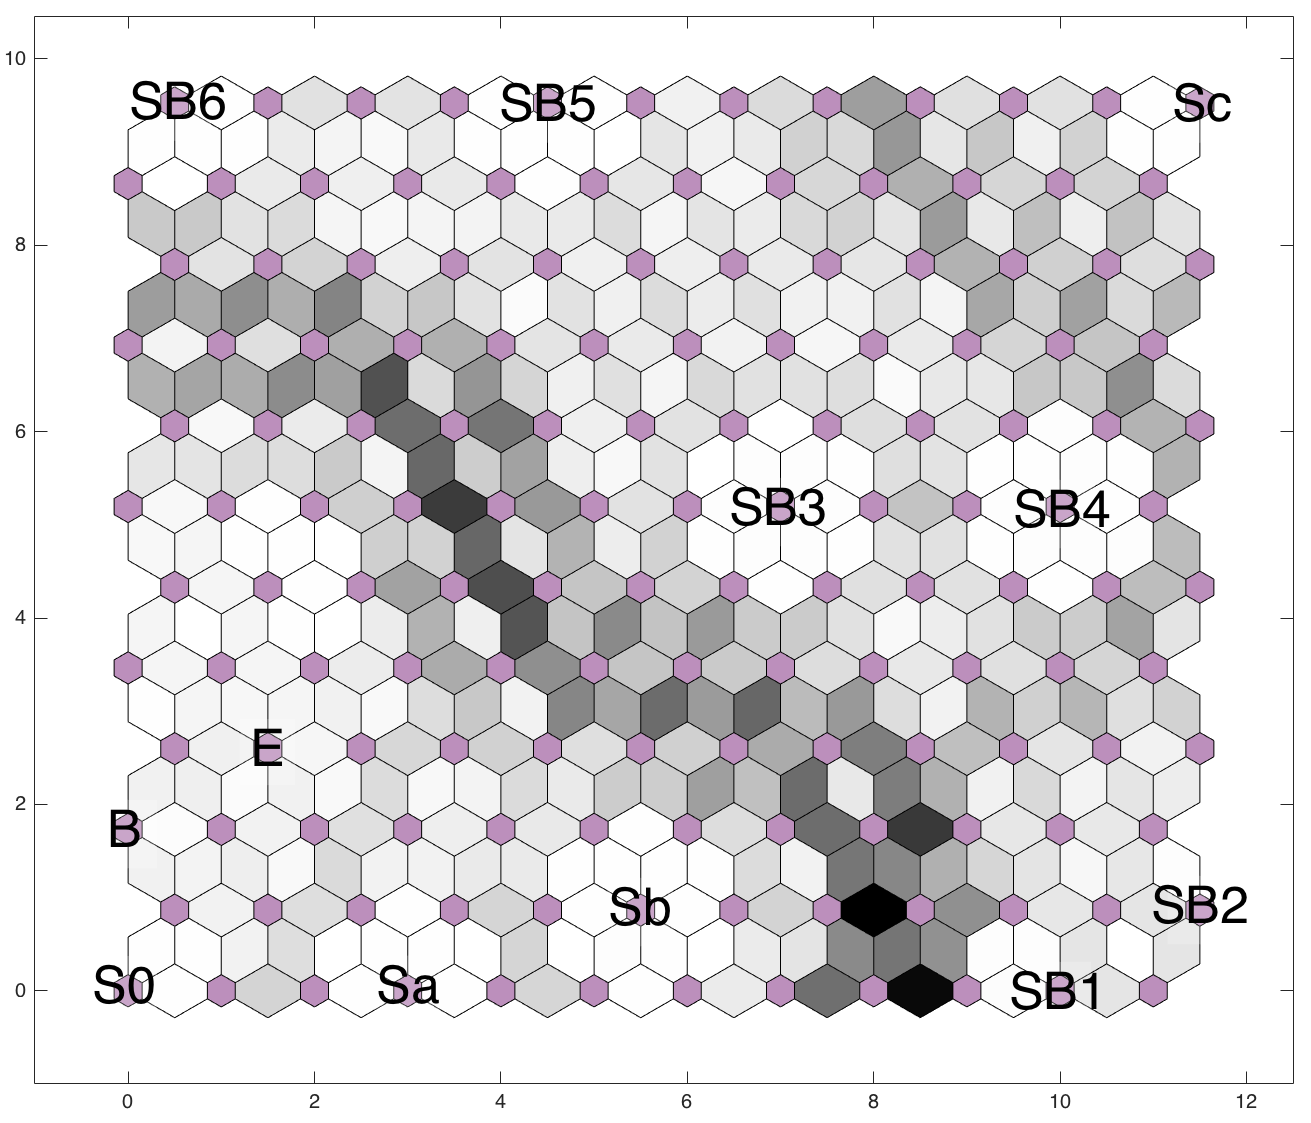
\includegraphics[width=\textwidth]{images0.01/2d/dist_12_by_12.png}
        \end{subfigure}
        \hfill
        \begin{subfigure}[b]{0.45\textwidth}
            \centering
            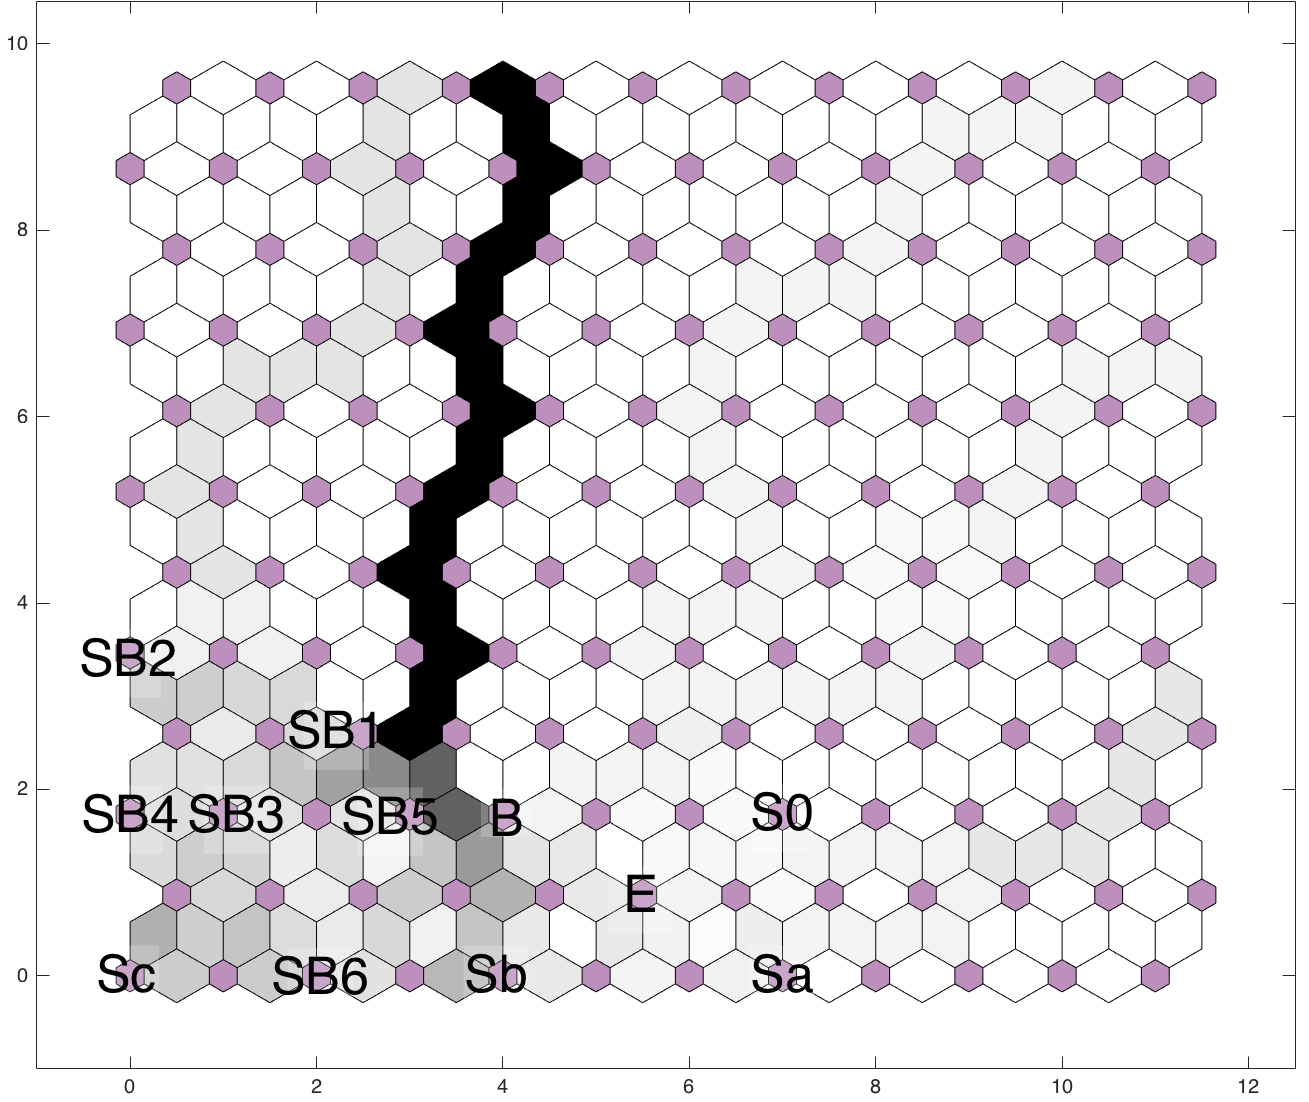
\includegraphics[width=\textwidth]{images0.01/2d/dist_12_by_self_org_res12.png}
        \end{subfigure}
        \hfill
        \begin{subfigure}[b]{0.45\textwidth}
            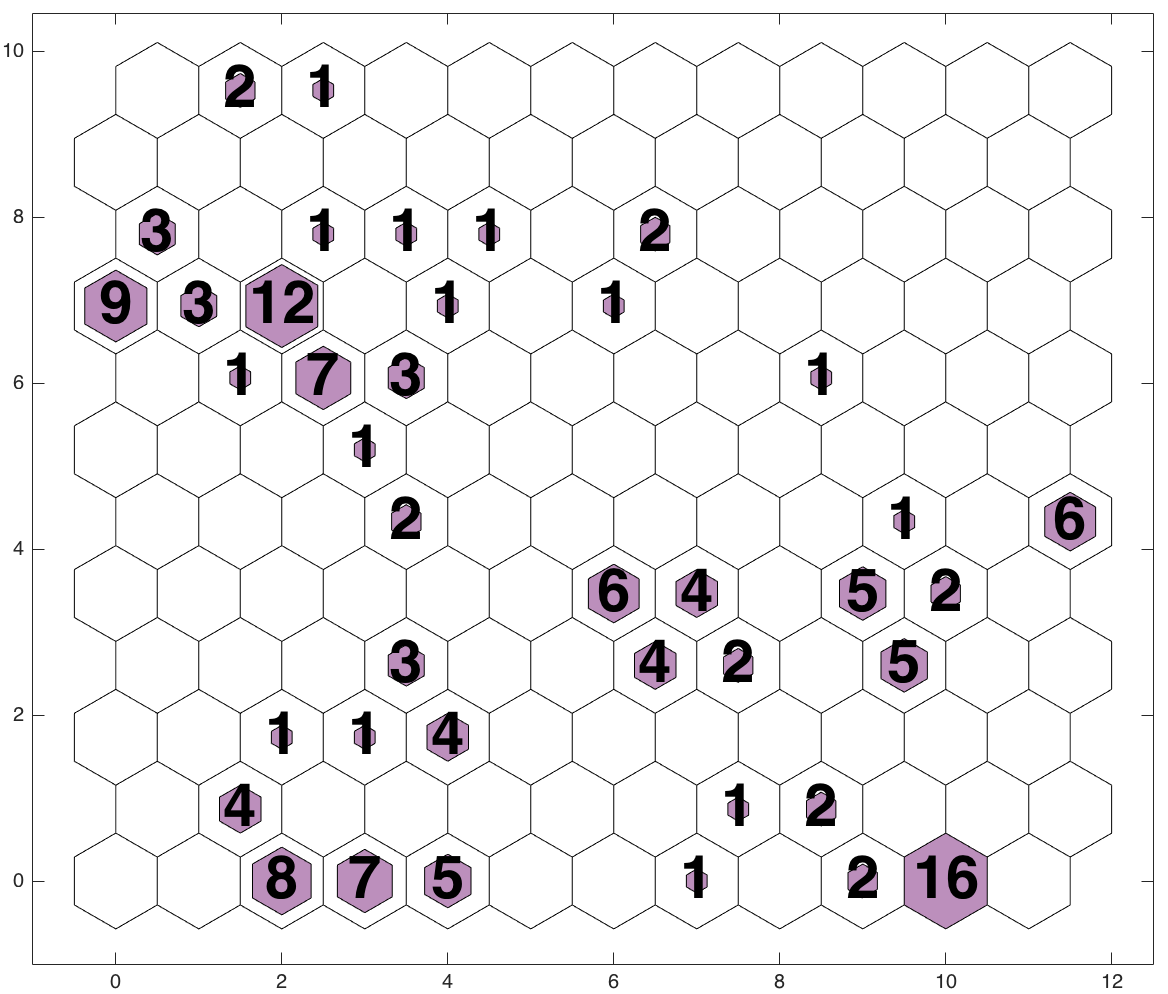
\includegraphics[width=\textwidth]{images0.01/2d/hit_v_12_by_12.png}
        \end{subfigure}
        \hfill
        \begin{subfigure}[b]{0.45\textwidth}
            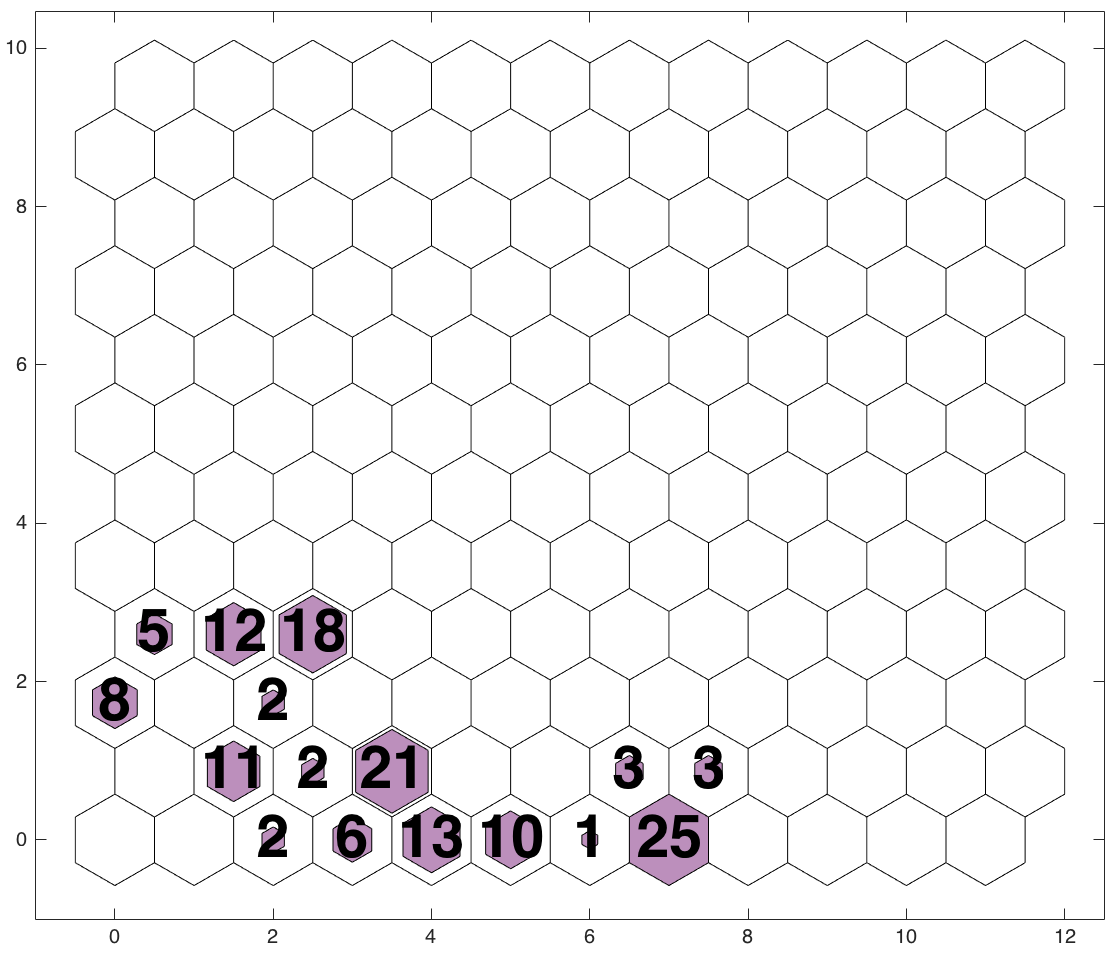
\includegraphics[width=\textwidth]{images0.01/2d/hit_v_12_by_self_org_res12.png}
        \end{subfigure}
        \caption{$12\times12$~2D SOM results. Up: Trained SOMs using K96. For training 2D SOMs two different approaches were considered; Either only 12 types of galaxies are existed (left) or not (right). Down: classifying the galaxies from T12, using the trained networks above them. From the right side one, we can see that there is no outlier in the galaxies from T12, and we can use the left side map as a final clustering results for the T12 galaxies.}
        \label{fig: 12by12}
    \end{figure*}
    
    The upper left part of Fig.~\ref{fig: 12by12} shows the SOM results from the first approach. 
    Since we considered that SEDs of all galaxies can be categorized using the K96 model, the galaxies took place all over the map.
    Using this network to categorize any set of SEDs, forced the SEDs to be in the same neurons as the K96 ones or the neurons between them.
    However, all the K96 galaxies are in small side of the map in the upper right map in Fig.~\ref{fig: 12by12}, which provide enough freedom for SED of the galaxies to take place everywhere in the map even it is way far away from the K96 templates.
    
    
    In the upper left part of the map in Fig.~\ref{fig: 12by12}, although galaxies have more space to move on and more can be separated in any way, they were separated in two main groups.
    There is a distinguishable strip of the grey, dark grey and in some cases black colour in the map.
    This strip is separating early type galaxies with starburst ones.
    The lower map shows that 5 of the neurons on the left side of the strip are full. 
    These five neurons are the same ones on the left hand side of Fig.~\ref{fig: 1by2T} (early type galaxies).
    The only difference is that here, in this map they have more space to be separated from each other.
    When we use this network to categorize the SED of galaxies, any galaxy places on the left hand side of the strip is an early type galaxy and anyone placed on the right side of the strip is a starburst one.
    The decision about what type of early type or starburst galaxy, is based upon its relative position to each type in the SOM.
    
    Same as other map, in the upper right map in Fig.~\ref{fig: 12by12}, galaxies generally are divided into two main groups.
    The border between the early type galaxies and the starburst ones is the black strips in the middle of the upper map, which end up with bright grey colour at the bottom of the map in the fifth neuron.
    In this network, neurons in the right side of the strip represent the early type galaxies and the neurons in the left side represent the starburst ones. 
    When categorizing a new set of SEDs, if the new SEDs are similar to K96 sample all of them will place in the bottom of the map, but if there are different type of the galaxies, they would sit in any other neurons in the map.
    In large data sets, one can easily used this network to figure out whether there is any new type of SEDs (or any outliers) are in the data sets or not. 
    Since, the networks are already available, this procedure should be really fast and easy for big data sets.
    
    We used the both 2D networks to categorize the T12 galaxies and showed the results in lower maps in Fig.~\ref{fig: 12by12}.
    Since in the lower right map in Fig.~\ref{fig: 12by12} all the galaxies placed in the bottom part of the map, we can conclude that there is no outlier or very different type of the SED from K96 templates in T12 samples.
    The lower left map of Fig.~\ref{fig: 12by12} represents the T12 galaxies categorization based on the network in the upper left of Fig.~\ref{fig: 12by12}. 
    Comparing this categorization with the 1D one from Fig.~\ref{fig: 1by22V}, we can see here, only 23 galaxies correspond exactly to K96 types.
    Using 2D maps, we categorized galaxies in more intermediate type than 1D ones.
    In both lower maps in Fig.~\ref{fig: 12by12}, most the galaxies are in the early type side of the SOM, which was predictable from the results in the Sec.\ref{sec: 1Dv}.
    Note that, from this sample we do not conclude that there are more early type galaxies in higher red-shifts.
    We simply indicate that in this sample, we have more early type galaxies, and the reason is the selection effect from the fact that those galaxies had more reliable redshift estimation. %PB20160510: could also talk about this as it relates to the method used to select the galaxies in the first place (once you find out what that was!)
    %SR20160512 I need to talk about it.
    
    Although because of the fluency of the paper, we first talked about 1D networks and continued to 2D networks we suggest that in case of using the SOMs to categorize the SED of the galaxies or to explore any related data, first step to be checking data using networks similar to the upper left map in Fig.~\ref{fig: 12by12}.
    In this case, all the outlier or specific cases would be identified and removed from the sample. 

    
    % \subsection{Caveat}
    % There is no established method to find the best SOM initial values. 
    % Size of the maps, number of neighbours in each steps, number of iterations could vary and each one give us a new results.
    % Also, since at the beginning the weights are generated randomly, in each run the results could have small differences.
    %no quantitative way to analyse the data?!
    
    
%----------------------------------------------------------------------------------------
%----------------------------------------------------------------------------------------
%----------------------------------------------------------------------------------------
%Summery
%----------------------------------------------------------------------------------------
%----------------------------------------------------------------------------------------
%----------------------------------------------------------------------------------------
\section{SUMMARY AND FUTURE APPLICATIONS}
\label{sec: summary}

Self organizing maps can be used to classify celestial objects (i.e. stars, quasars, spectra of galaxies, light curves, etc.).
We showed that we can create various networks with different sizes/dimensions based on information we need from the data. 
If a broad and general classification is required, networks can have one dimension with few number of neurons.
While if we need classifications based on differences in more details, we can use a higher number of neurons.
Since the SOM codes does not work with uncertainty of input parameter, sometimes too much attention to details can cause problems in classifications. 
Some small differences could easily be the result of atmosphere fluctuation or other instrumental or observational problems. 
for using SOM method, one should be careful about these small differences and consider in order to separate two groups from each other, how much details do they need to pay attention to.

We used SOMs to classify SEDs of the galaxies with known morphological type from K96, and created networks with different usages.
By varying size of networks, we found the relative similarity or dissimilarity between each type of galaxies.
since we needed a 1D network with 22 neurons to be able to separate all the 12 types of galaxies from K96 for the first time, we concluded that types B and E, and types SB1 and SB2 galaxies are really similar to each other.
We also showed that networks generated with SOM method can be used to easily identified new type of the galaxies or outlier, in large surveys.

The sample of 142 high red-shift galaxies from T12 was used to test the trained networks.
One of the main criteria to chose a test sample is that the test sample must have fluxes in exactly the same wavelengths of the training sample.
The test results showed that using SOMs can lead us to identify galaxies with SEDs similar to two or more morphological types but not exactly the same as one of them.
A freedom of having in between types is one of the main differences between supervised and unsupervised ANNs.
T12  have used a supervised training method, and trained networks with K96 SED template.
Same as this project, they tried to classify the sample of 142 galaxies using the trained networks.
However, they could not classify 37 out of 142 galaxies in the sample.
The unsupervised method that we used in this project, gave us the ability to classify galaxies either as one of the morphological types that have been introduced by K96 or between those types. 
Therefore, we classified all 142 galaxies of our test sample.
We plotted the properties of the galaxies in test sample using new classification and found a tighter correlations between mean values of age, sSFR, stellar mass, and extinction in FUV band of the galaxies in new classifications than previous studies.
We also showed he properties of the galaxies in each groups is in good agreement between their morphological types.


\section*{ACKNOWLEDGMENTS}
S.R. and P.B. acknowledge research support from the Natural Sciences and Engineering Research Council of Canada. 
%----------------------------------------------------------------------------------------
%----------------------------------------------------------------------------------------
%----------------------------------------------------------------------------------------
%biblio
%----------------------------------------------------------------------------------------
%----------------------------------------------------------------------------------------
%----------------------------------------------------------------------------------------
\bibliographystyle{mnras}
\bibliography{ref_mining_h.bib}

\import{sections0.0/}{apps0.0.tex}
\end{document}
